\documentclass[a4paper]{article}

% CJK support: prefer ctex, fallback to XeTeX native line breaking
\IfFileExists{ctex.sty}{
  \usepackage[fontset=fandol]{ctex}
}{
  % Fallback for minimal TeX installs (e.g. MacTeX Basic, TeX Live scheme-basic)
  % without ctex/xeCJK. Uses XeTeX's built-in CJK line breaking.
  \usepackage{fontspec}
  \XeTeXlinebreaklocale "zh"
  \XeTeXlinebreakskip = 0pt plus 1pt
  \IfFontExistsTF{Songti SC}{\setmainfont{Songti SC}}{%
    \IfFontExistsTF{Noto Serif CJK SC}{\setmainfont{Noto Serif CJK SC}}{}%
  }
  \IfFontExistsTF{Heiti SC}{\setsansfont{Heiti SC}}{%
    \IfFontExistsTF{Noto Sans CJK SC}{\setsansfont{Noto Sans CJK SC}}{}%
  }
}

% Basic packages
\usepackage{amsmath, amssymb}
\usepackage{graphicx}
\usepackage[margin=2.5cm]{geometry}
\emergencystretch=3em
\usepackage[most]{tcolorbox}
\usepackage{etoolbox}
\usepackage{listings}
\usepackage{hyperref}
\usepackage{booktabs}
\usepackage{array}
\usepackage{subcaption}
\usepackage{float}
\usepackage{tikz}
\IfFileExists{pgfplots.sty}{
    \usepackage{pgfplots}
    \pgfplotsset{compat=1.18}
}{}

% ===== Highlight boxes =====
\newtcolorbox{knowledgebox}[1]{
    enhanced, colback=blue!5!white, colframe=blue!75!black, colbacktitle=blue!75!black,
    coltitle=white, fonttitle=\bfseries, title={#1}, attach boxed title to top left={yshift=-2mm, xshift=2mm},
    boxrule=1pt, sharp corners
}

\newtcolorbox{importantbox}[1]{
    enhanced, colback=yellow!10!white, colframe=yellow!80!black, colbacktitle=yellow!80!black,
    coltitle=black, fonttitle=\bfseries, title={#1}, sharp corners
}

\newtcolorbox{warningbox}[1]{
    enhanced, colback=red!5!white, colframe=red!75!black, colbacktitle=red!75!black,
    coltitle=white, fonttitle=\bfseries, title={#1}, sharp corners
}

\newtcolorbox{practicebox}[1]{
    enhanced, colback=black!3!white, colframe=black!75, colbacktitle=black!75,
    coltitle=white, fonttitle=\bfseries, title={#1}, sharp corners
}

% ===== Code listings =====
\lstset{
    basicstyle=\ttfamily\small,
    keywordstyle=\color{blue},
    stringstyle=\color{red!60!black},
    commentstyle=\color{green!60!black},
    breaklines=true,
    frame=single,
    numbers=left,
    numberstyle=\tiny\color{gray},
    captionpos=b,
    extendedchars=false
}

% ===== Figure provenance and unit macros =====
% \vtag goes inside \caption{...}; \srcnote{MM:SS--MM:SS} follows the figure environment.
\newcommand{\vtag}{\protect\footnotemark}
\newcommand{\srcnote}[1]{\footnotetext{视频画面时间区间：#1。若为裁剪图，时间区间仍对应原视频画面。}}
% Units work in text and math mode; never hand-write $^\circ$ or \AA inside \mathrm.
\newcommand{\degC}{\ensuremath{^{\circ}\mathrm{C}}}
\newcommand{\um}{\ensuremath{\mu\mathrm{m}}}
\newcommand{\nm}{\ensuremath{\mathrm{nm}}}
\newcommand{\angstrom}{\ensuremath{\text{\AA}}}

% ===== Front-page metadata =====
% Fill these in when generating notes.
\newcommand{\notetitle}{古典微分几何}
\newcommand{\notesubtitle}{GAMES001 图形学中的数学 · 第 11 集：曲线论与曲面论}
\newcommand{\noteauthors}{根据 GAMES-Webinar 直播录像整理（倪星宇 主讲）}
\newcommand{\notedate}{2024年5月27日（直播）}
\newcommand{\videochannel}{GAMES-Webinar（哔哩哔哩）}
\newcommand{\videopublishdate}{2024年3月6日（合集）}
\newcommand{\videoduration}{1小时22分30秒}
\newcommand{\videourl}{https://www.bilibili.com/video/BV1MF4m1V7e3/?p=11}
\newcommand{\videocoverpath}{cover.jpg}

\begin{document}

% ===== Title page =====
\begin{titlepage}
\centering
{\Large 课程笔记\par}
\vspace{1.2cm}
{\huge\bfseries \notetitle\par}
\ifdefempty{\notesubtitle}{}{
\vspace{0.3cm}
{\large \notesubtitle\par}
}
\vspace{0.5cm}
{\large \noteauthors\par}
\vspace{0.3cm}
{\large \notedate\par}
\vspace{1.0cm}

\ifdefempty{\videocoverpath}{
{\small 请在生成笔记时填入视频封面图的本地路径。\par}
}{
\includegraphics[width=0.82\textwidth,height=0.40\textheight,keepaspectratio]{\videocoverpath}\par
}

\vfill
\begin{tcolorbox}[width=0.9\textwidth, colback=black!2!white, colframe=black!60, sharp corners]
\textbf{视频作者/频道}：\videochannel\par
\textbf{发布日期}：\videopublishdate\par
\textbf{视频时长}：\videoduration\par
\textbf{视频链接}：
\ifdefempty{\videourl}{
未填写
}{
\href{\videourl}{\nolinkurl{\videourl}}
}
\end{tcolorbox}
\end{titlepage}

\tableofcontents
\newpage

%% --- 正文内容开始 --- %%

\section{这一讲讲什么}

第十一讲由倪星宇主讲，主题是古典微分几何（classical differential geometry）。讲者先解释为什么微分几何有“古典”的说法：古典微分几何是和现代微分几何相对的。古典微分几何是一种外蕴方法，研究镶嵌在三维空间中的二维曲面；研究对象主要为曲面，概念和方法从曲线派生，故又称为曲线与曲面论。现代微分几何是内蕴方法，它不是站在超越流形或曲面的空间中，而是站在流形之内研究任意维度的流形本身；研究对象是各种流形，更多是我们无法在三维空间中想象的那种，广泛应用于广义相对论等研究中。

那么微分几何与图形学有什么关系？图形学的研究对象是 $\mathbb R^3$ 空间的可视化呈现：空间里有各种各样的几何体，要把它们和它们的运动画出来，图形学无非就是在干这样的事，而这恰好对应于古典微分几何的范畴。所以做图形学研究，很多时候需要一些古典微分几何的知识。

本讲分为两大部分：曲线论（参数曲线、弧长、曲率与挠率、Frenet 标架、曲线论基本定理、近似展开）和曲面论（参数曲面、切平面与法线、第一与第二基本形、保长与保角、可展曲面、曲面的曲率、曲面论基本定理），最后讲几何连续性。

\begin{importantbox}{本讲的主线}
曲线由两个数决定形状：曲率和挠率；曲面由两个“基本形”决定形状：第一基本形度量长度、角度和面积，第二基本形度量弯曲。曲面的各种曲率（法曲率、主曲率、平均曲率、高斯曲率）都可以由这两个基本形算出。而高斯绝妙定理指出，高斯曲率只依赖第一基本形，这是从古典微分几何通向现代微分几何的关键一步。
\end{importantbox}

\noindent\begin{minipage}{\textwidth}
\begin{figure}[H]
\centering
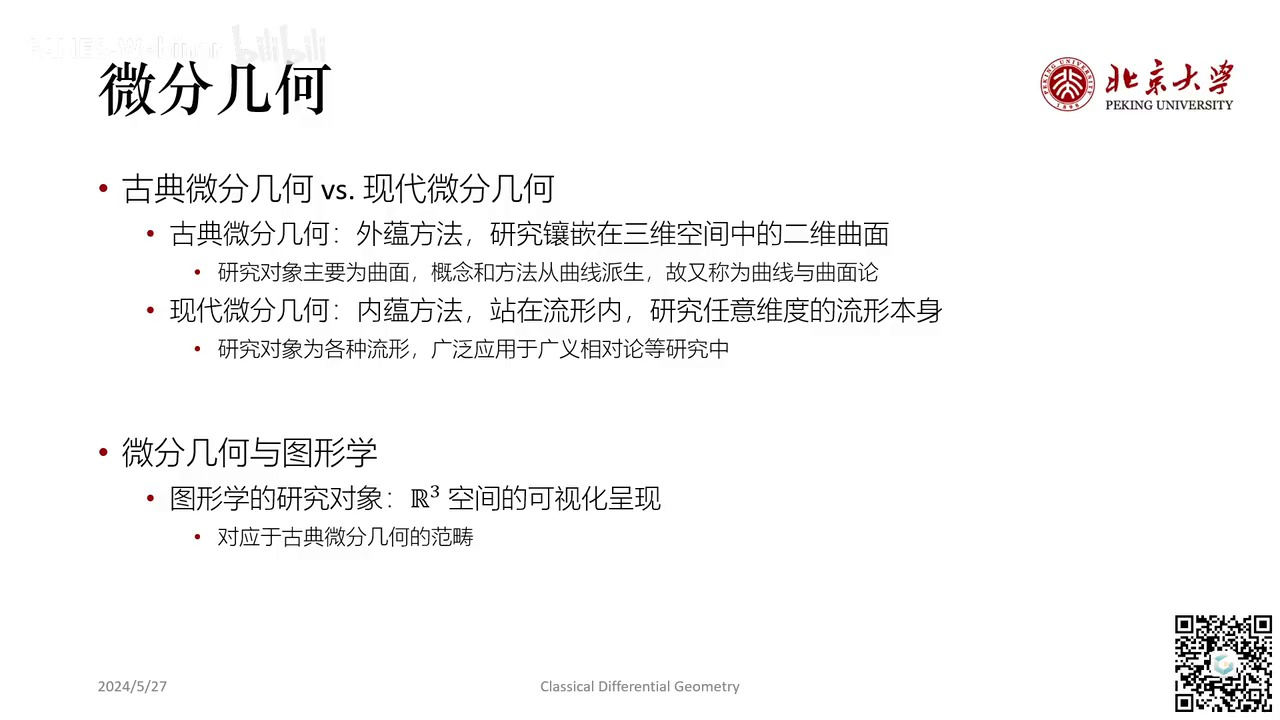
\includegraphics[width=0.92\textwidth]{figures/fig_01_intro.jpg}
\caption{古典微分几何与现代微分几何，以及微分几何与图形学的关系\vtag}
\end{figure}
\srcnote{00:02:45--00:03:00}
\end{minipage}


\section{参数曲线}

\subsection{曲线与参数曲线}

\noindent\begin{minipage}{\textwidth}
\begin{figure}[H]
\centering
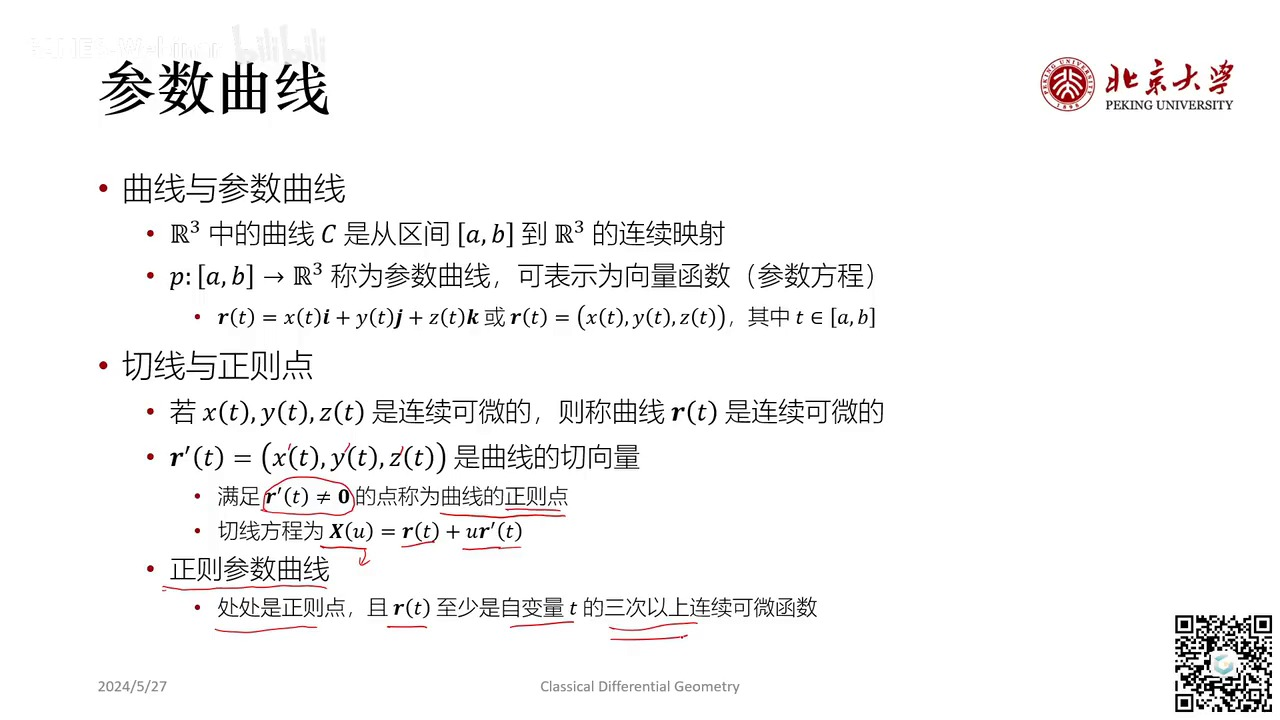
\includegraphics[width=0.92\textwidth]{figures/fig_02_curve.jpg}
\caption{曲线与参数曲线、切线与正则点\vtag}
\end{figure}
\srcnote{00:05:00--00:05:15}
\end{minipage}


在三维欧几里得空间中，曲线和我们在纸上画的曲线不一样，它的走向可能并不在一个平面里。所以用一个连续映射来表示曲线：$\mathbb R^3$ 中的曲线 $C$ 是从区间 $[a,b]$ 到 $\mathbb R^3$ 的连续映射。$\boldsymbol p:[a,b]\to\mathbb R^3$ 称为参数曲线，可表示为向量函数（参数方程）
\begin{equation}
\boldsymbol r(t)=x(t)\boldsymbol i+y(t)\boldsymbol j+z(t)\boldsymbol k=\big(x(t),y(t),z(t)\big),\qquad t\in[a,b].
\end{equation}

\subsection{切线与正则点}

若 $x(t),y(t),z(t)$ 是连续可微的，则称曲线 $\boldsymbol r(t)$ 是连续可微的。$\boldsymbol r'(t)=\big(x'(t),y'(t),z'(t)\big)$ 是曲线的切向量。满足 $\boldsymbol r'(t)\ne\boldsymbol 0$ 的点称为曲线的正则点，切线方程为 $\boldsymbol X(u)=\boldsymbol r(t)+u\boldsymbol r'(t)$。处处是正则点，且 $\boldsymbol r(t)$ 至少是自变量 $t$ 的三次以上连续可微函数的曲线，称为正则参数曲线。

讲者解释为什么要求“三次以上”：后面会看到，曲线论中要考察曲率和挠率，挠率需要用到三阶导数，所以曲线需要具有一定程度的连续可微性。

\subsection{弧长与弧长参数}

\noindent\begin{minipage}{\textwidth}
\begin{figure}[H]
\centering
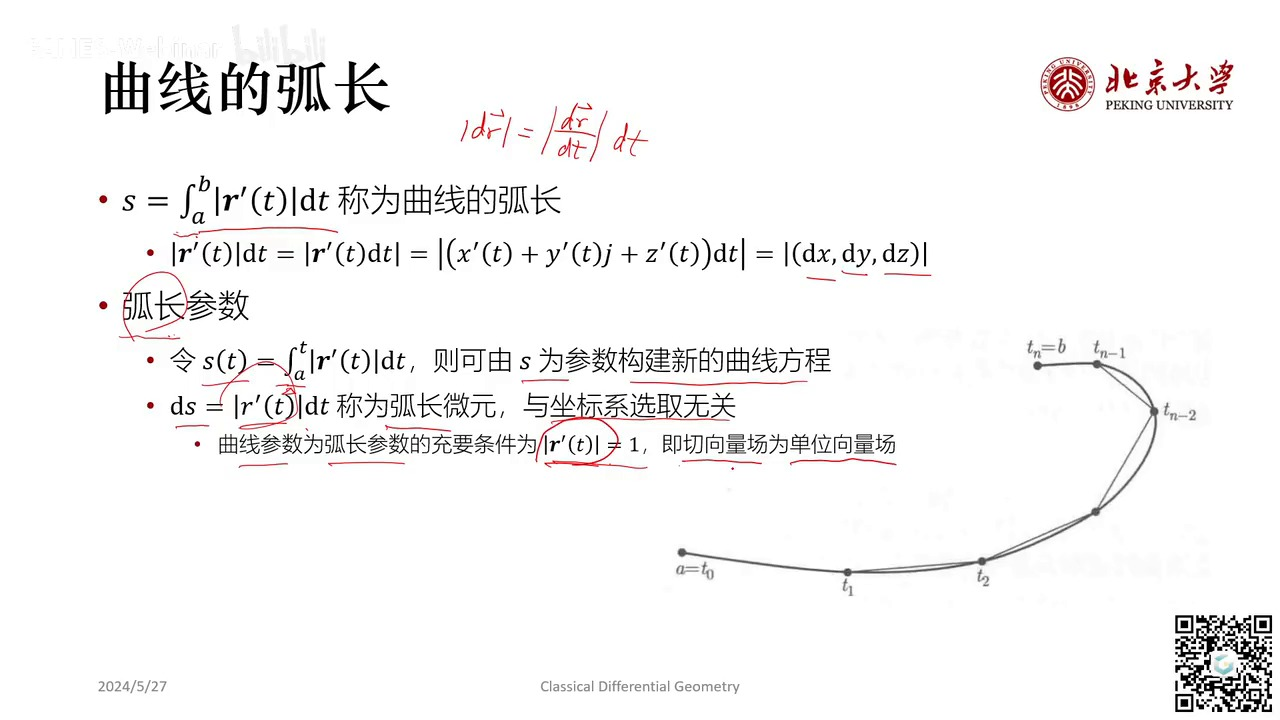
\includegraphics[width=0.92\textwidth]{figures/fig_03_arclength.jpg}
\caption{曲线的弧长与弧长参数\vtag}
\end{figure}
\srcnote{00:07:15--00:07:30}
\end{minipage}


曲线的弧长定义为
\begin{equation}
s=\int_a^b|\boldsymbol r'(t)|\,\mathrm{d}t,
\end{equation}
其中 $|\boldsymbol r'(t)|\mathrm{d}t=|\boldsymbol r'(t)\mathrm{d}t|=|(x'(t)\boldsymbol i+y'(t)\boldsymbol j+z'(t)\boldsymbol k)\mathrm{d}t|=|(\mathrm{d}x,\mathrm{d}y,\mathrm{d}z)|$，也可以把它还原回 $\mathrm{d}x,\mathrm{d}y,\mathrm{d}z$ 的形式。右图把曲线用折线逼近，折线长度的极限就是弧长。

令 $s(t)=\int_a^t|\boldsymbol r'(t)|\,\mathrm{d}t$，就可以以 $s$ 为参数构建新的曲线方程。$\mathrm{d}s=|\boldsymbol r'(t)|\,\mathrm{d}t$ 称为弧长微元，它与坐标系的选取无关。曲线参数为弧长参数的充要条件为 $|\boldsymbol r'(s)|=1$，即切向量场为单位向量场。

\begin{knowledgebox}{为什么偏爱弧长参数}
同一条曲线可以有无穷多种参数化，参数走得快慢不同，$\boldsymbol r'(t)$ 的长度也不同。弧长参数相当于“匀速走”，切向量恒为单位长度，于是导数的变化只反映曲线本身的弯曲，而不混入参数化的快慢。后面的曲率、挠率都先在弧长参数下定义，再换算到一般参数。
\end{knowledgebox}

\section{曲率与挠率}

\subsection{曲率与主法向量}

\noindent\begin{minipage}{\textwidth}
\begin{figure}[H]
\centering
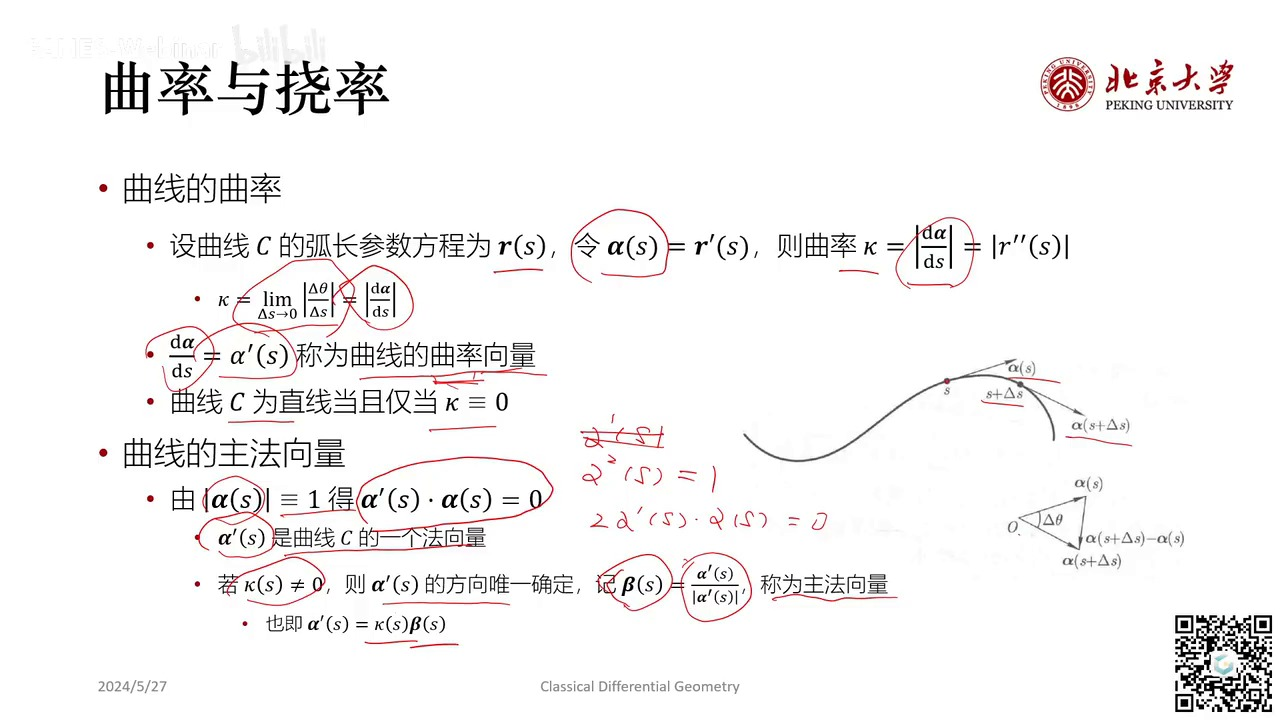
\includegraphics[width=0.92\textwidth]{figures/fig_04_curvature.jpg}
\caption{曲线的曲率与主法向量\vtag}
\end{figure}
\srcnote{00:11:15--00:11:30}
\end{minipage}


设曲线 $C$ 的弧长参数方程为 $\boldsymbol r(s)$，令 $\boldsymbol\alpha(s)=\boldsymbol r'(s)$ 为单位切向量，则曲率
\begin{equation}
\kappa=\left|\frac{\mathrm{d}\boldsymbol\alpha}{\mathrm{d}s}\right|=|\boldsymbol r''(s)|=\lim_{\Delta s\to 0}\left|\frac{\Delta\theta}{\Delta s}\right| .
\end{equation}
它的几何意义是：沿着曲线走的时候，切向量转过的角度 $\Delta\theta$ 与走过的弧长 $\Delta s$ 之比。$\frac{\mathrm{d}\boldsymbol\alpha}{\mathrm{d}s}=\boldsymbol\alpha'(s)$ 称为曲线的曲率向量。曲线 $C$ 为直线当且仅当 $\kappa\equiv 0$。

由 $|\boldsymbol\alpha(s)|\equiv 1$，两边对 $s$ 求导得 $2\boldsymbol\alpha'(s)\cdot\boldsymbol\alpha(s)=0$，即 $\boldsymbol\alpha'(s)\cdot\boldsymbol\alpha(s)=0$，所以 $\boldsymbol\alpha'(s)$ 是曲线 $C$ 的一个法向量。若 $\kappa(s)\ne 0$，则 $\boldsymbol\alpha'(s)$ 的方向唯一确定，记
\begin{equation}
\boldsymbol\beta(s)=\frac{\boldsymbol\alpha'(s)}{|\boldsymbol\alpha'(s)|},
\end{equation}
称为主法向量，也即 $\boldsymbol\alpha'(s)=\kappa(s)\boldsymbol\beta(s)$。

\subsection{Frenet 标架}

\noindent\begin{minipage}{\textwidth}
\begin{figure}[H]
\centering
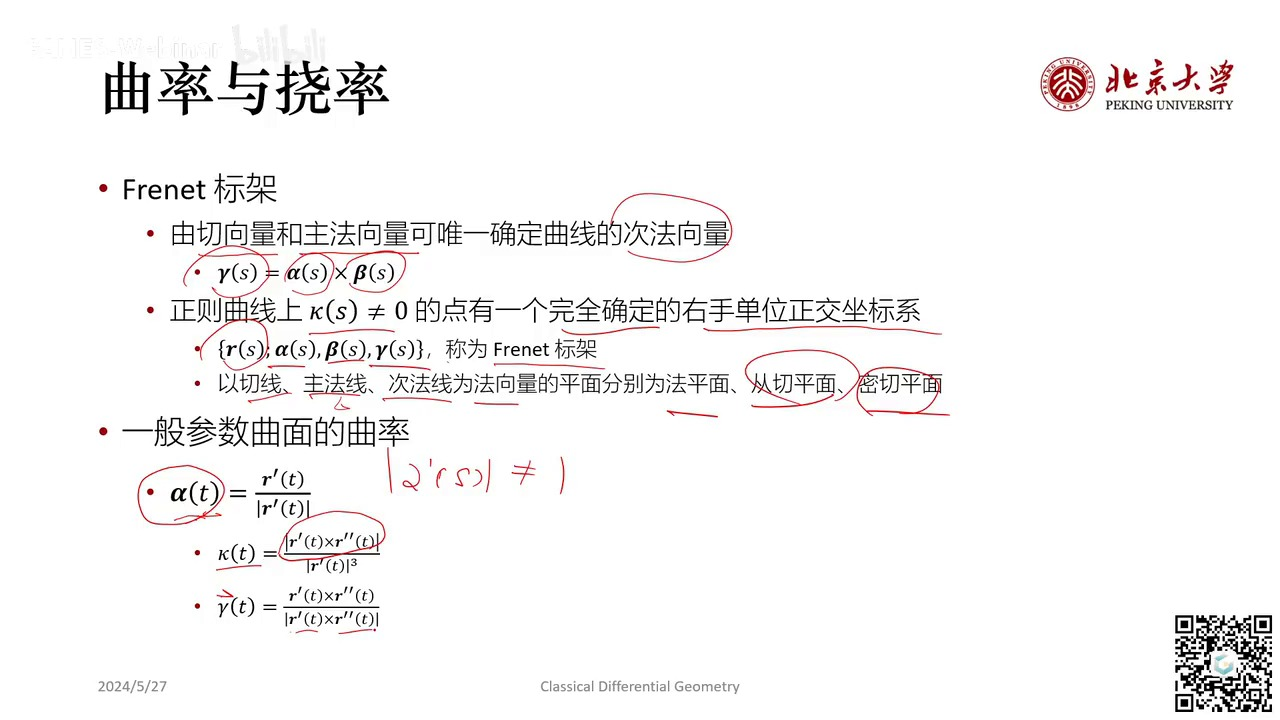
\includegraphics[width=0.92\textwidth]{figures/fig_05_frenet.jpg}
\caption{Frenet 标架与一般参数曲线的曲率\vtag}
\end{figure}
\srcnote{00:13:45--00:14:00}
\end{minipage}


由切向量和主法向量可唯一确定曲线的次法向量 $\boldsymbol\gamma(s)=\boldsymbol\alpha(s)\times\boldsymbol\beta(s)$。正则曲线上 $\kappa(s)\ne 0$ 的点有一个完全确定的右手单位正交坐标系 $\{\boldsymbol r(s);\boldsymbol\alpha(s),\boldsymbol\beta(s),\boldsymbol\gamma(s)\}$，称为 Frenet 标架，原点就在曲线上的点 $\boldsymbol r(s)$。以切线、主法线、次法线为法向量的平面分别为法平面、从切平面、密切平面。

如果是一般参数曲线，参数 $t$ 不满足 $|\boldsymbol r'(t)|=1$，则
\begin{equation}
\boldsymbol\alpha(t)=\frac{\boldsymbol r'(t)}{|\boldsymbol r'(t)|},\qquad \kappa(t)=\frac{|\boldsymbol r'(t)\times\boldsymbol r''(t)|}{|\boldsymbol r'(t)|^3},\qquad \boldsymbol\gamma(t)=\frac{\boldsymbol r'(t)\times\boldsymbol r''(t)}{|\boldsymbol r'(t)\times\boldsymbol r''(t)|}.
\end{equation}

\subsection{挠率}

\noindent\begin{minipage}{\textwidth}
\begin{figure}[H]
\centering
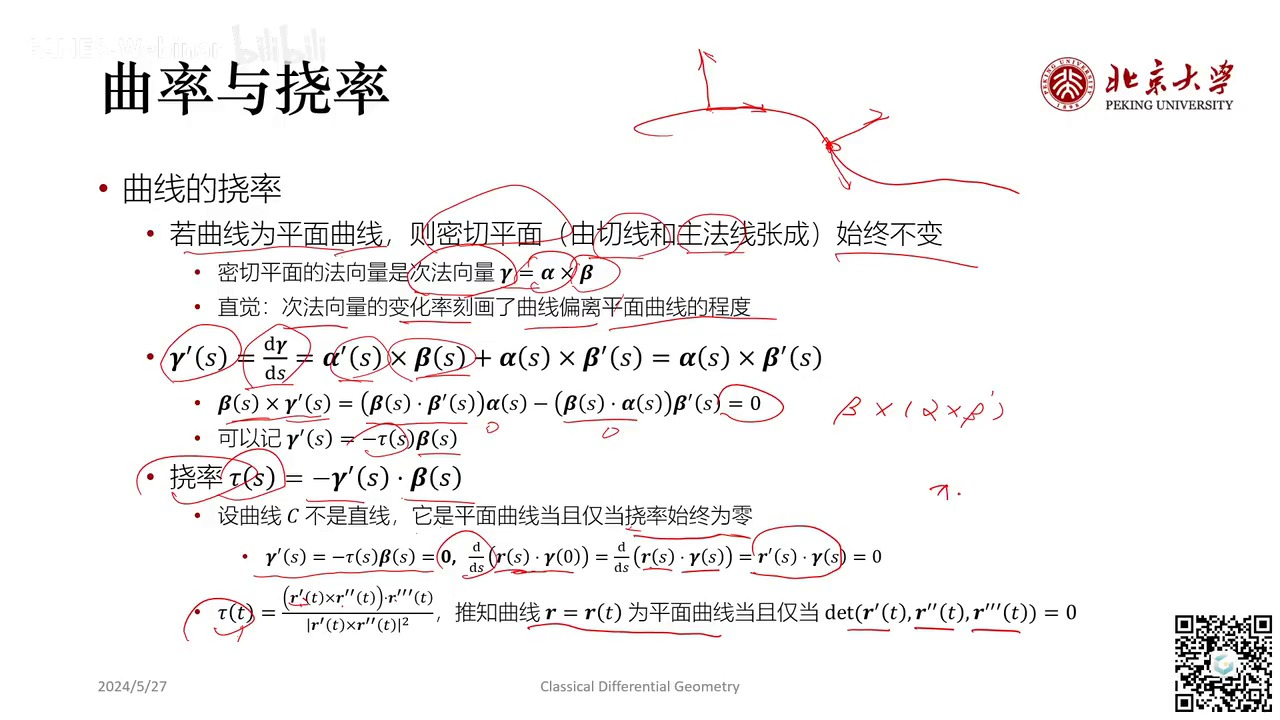
\includegraphics[width=0.92\textwidth]{figures/fig_06_torsion.jpg}
\caption{曲线的挠率\vtag}
\end{figure}
\srcnote{00:19:45--00:20:00}
\end{minipage}


若曲线为平面曲线，则密切平面（由切线和主法线张成）始终不变。讲者解释：如果曲线画在纸面上，每一点的主法线和切线全都在纸面内，所以密切平面就是纸面。密切平面的法向量是次法向量 $\boldsymbol\gamma=\boldsymbol\alpha\times\boldsymbol\beta$，所以直观上，次法向量的变化率刻画了曲线偏离平面曲线的程度。计算
\begin{equation}
\boldsymbol\gamma'(s)=\frac{\mathrm{d}\boldsymbol\gamma}{\mathrm{d}s}=\boldsymbol\alpha'(s)\times\boldsymbol\beta(s)+\boldsymbol\alpha(s)\times\boldsymbol\beta'(s)=\boldsymbol\alpha(s)\times\boldsymbol\beta'(s),
\end{equation}
因为 $\boldsymbol\alpha'$ 与 $\boldsymbol\beta$ 平行，第一项为零。再用二重叉积展开：
\begin{equation}
\boldsymbol\beta(s)\times\boldsymbol\gamma'(s)=\big(\boldsymbol\beta(s)\cdot\boldsymbol\beta'(s)\big)\boldsymbol\alpha(s)-\big(\boldsymbol\beta(s)\cdot\boldsymbol\alpha(s)\big)\boldsymbol\beta'(s)=\boldsymbol 0,
\end{equation}
因为 $\boldsymbol\beta$ 是单位向量，$\boldsymbol\beta\cdot\boldsymbol\beta'=0$，且 $\boldsymbol\beta\cdot\boldsymbol\alpha=0$。所以 $\boldsymbol\gamma'$ 与 $\boldsymbol\beta$ 平行，可以记 $\boldsymbol\gamma'(s)=-\tau(s)\boldsymbol\beta(s)$。称
\begin{equation}
\tau(s)=-\boldsymbol\gamma'(s)\cdot\boldsymbol\beta(s)
\end{equation}
为挠率。

设曲线 $C$ 不是直线，它是平面曲线当且仅当挠率始终为零：若 $\boldsymbol\gamma'(s)=-\tau(s)\boldsymbol\beta(s)\equiv\boldsymbol 0$，则 $\frac{\mathrm{d}}{\mathrm{d}s}\big(\boldsymbol r(s)\cdot\boldsymbol\gamma(0)\big)=\boldsymbol r'(s)\cdot\boldsymbol\gamma(0)=0$，曲线始终在一个平面内。对一般参数，
\begin{equation}
\tau(t)=\frac{\big(\boldsymbol r'(t)\times\boldsymbol r''(t)\big)\cdot\boldsymbol r'''(t)}{|\boldsymbol r'(t)\times\boldsymbol r''(t)|^2},
\end{equation}
推知曲线为平面曲线当且仅当 $\det\big(\boldsymbol r'(t),\boldsymbol r''(t),\boldsymbol r'''(t)\big)=0$。

\subsection{Frenet 公式}

\noindent\begin{minipage}{\textwidth}
\begin{figure}[H]
\centering
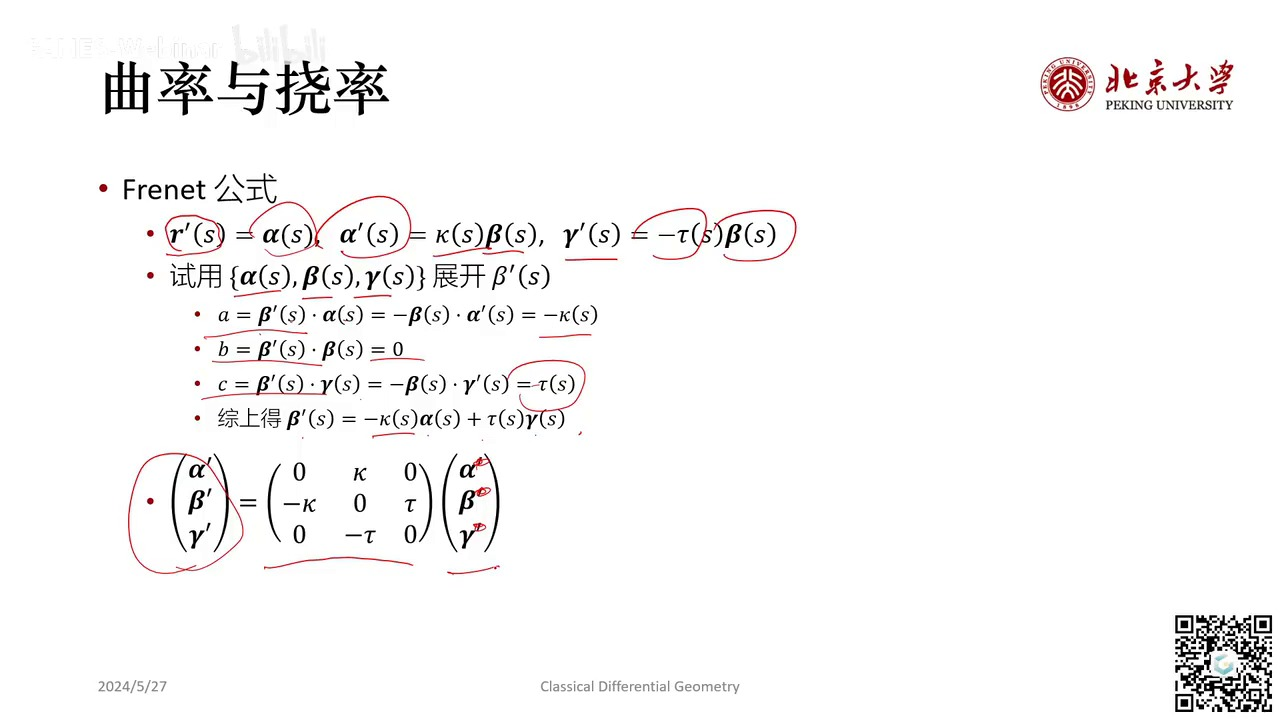
\includegraphics[width=0.92\textwidth]{figures/fig_07_frenet_formula.jpg}
\caption{Frenet 公式及其矩阵形式\vtag}
\end{figure}
\srcnote{00:22:00--00:22:15}
\end{minipage}


现在可以在 Frenet 标架下用基底 $\{\boldsymbol\alpha,\boldsymbol\beta,\boldsymbol\gamma\}$ 展开 $\boldsymbol\beta'(s)=a\boldsymbol\alpha+b\boldsymbol\beta+c\boldsymbol\gamma$：
\begin{equation}
\begin{gathered}
a=\boldsymbol\beta'\cdot\boldsymbol\alpha=-\boldsymbol\beta\cdot\boldsymbol\alpha'=-\kappa,\qquad b=\boldsymbol\beta'\cdot\boldsymbol\beta=0,\qquad c=\boldsymbol\beta'\cdot\boldsymbol\gamma=-\boldsymbol\beta\cdot\boldsymbol\gamma'=\tau,
\end{gathered}
\end{equation}
综上得 $\boldsymbol\beta'(s)=-\kappa(s)\boldsymbol\alpha(s)+\tau(s)\boldsymbol\gamma(s)$。与前面的结果合起来，就是 Frenet 公式：
\begin{equation}
\begin{pmatrix}\boldsymbol\alpha'\\ \boldsymbol\beta'\\ \boldsymbol\gamma'\end{pmatrix}=
\begin{pmatrix}0&\kappa&0\\-\kappa&0&\tau\\0&-\tau&0\end{pmatrix}
\begin{pmatrix}\boldsymbol\alpha\\ \boldsymbol\beta\\ \boldsymbol\gamma\end{pmatrix}.
\end{equation}
讲者指出，标架本身沿着曲线的运动方程就由这个反对称矩阵给出。

\begin{knowledgebox}{反对称矩阵与转动}
讲义作者补充：系数矩阵是反对称的并非巧合。$\{\boldsymbol\alpha,\boldsymbol\beta,\boldsymbol\gamma\}$ 始终是单位正交标架，它沿曲线的变化只能是一个转动；第四讲讲过，转动的“导数”是反对称矩阵，对应角速度。这里的角速度向量是 $\tau\boldsymbol\alpha+\kappa\boldsymbol\gamma$，常称为 Darboux 向量。
\end{knowledgebox}

\section{曲线论基本定理与近似展开}

\subsection{曲线论基本定理}

\noindent\begin{minipage}{\textwidth}
\begin{figure}[H]
\centering
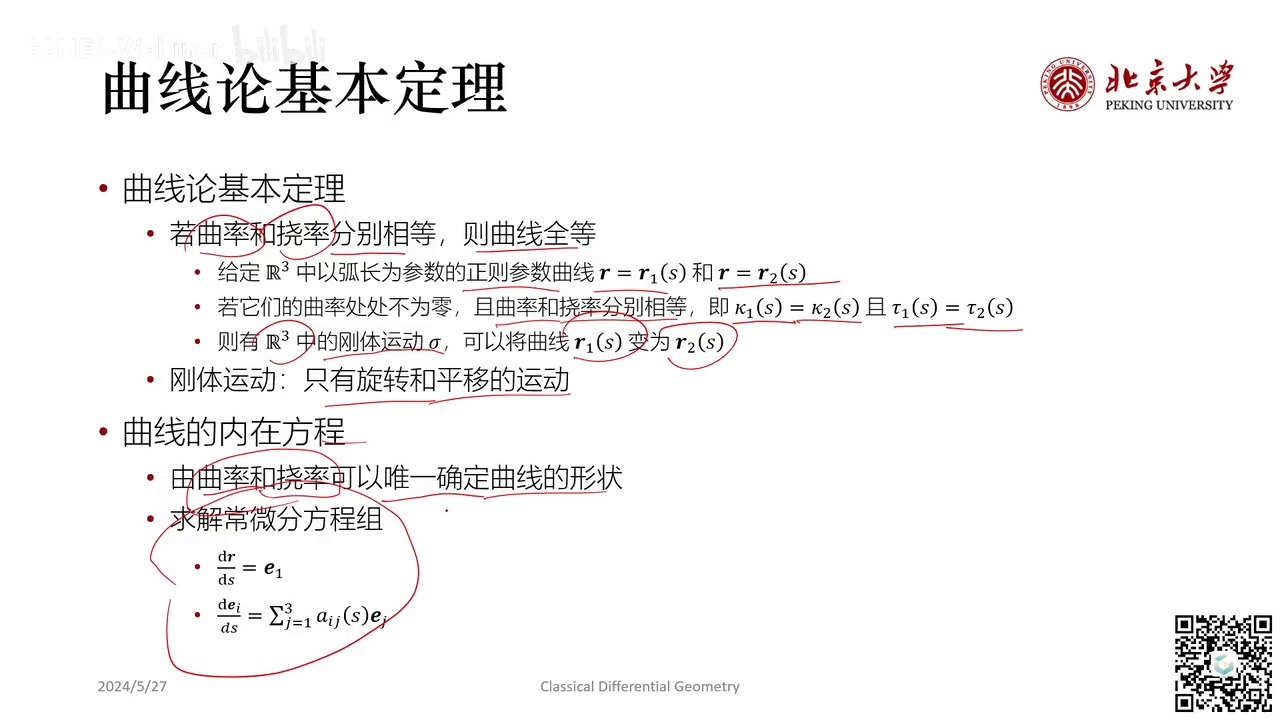
\includegraphics[width=0.92\textwidth]{figures/fig_08_curve_theorem.jpg}
\caption{曲线论基本定理与曲线的内在方程\vtag}
\end{figure}
\srcnote{00:23:45--00:24:00}
\end{minipage}


若曲率和挠率分别相等，则曲线全等。给定 $\mathbb R^3$ 中以弧长为参数的正则参数曲线 $\boldsymbol r=\boldsymbol r_1(s)$ 和 $\boldsymbol r=\boldsymbol r_2(s)$，若它们的曲率处处不为零，且曲率和挠率分别相等，即 $\kappa_1(s)=\kappa_2(s)$ 且 $\tau_1(s)=\tau_2(s)$，则在 $\mathbb R^3$ 中一定存在刚体运动 $\sigma$，可以将曲线 $\boldsymbol r_1(s)$ 变为 $\boldsymbol r_2(s)$。刚体运动只有旋转和平移的运动，所以两条曲线在形状上完全相同。

反过来，曲线的内在方程：由曲率和挠率可以唯一确定曲线的形状，只需求解常微分方程组
\begin{equation}
\frac{\mathrm{d}\boldsymbol r}{\mathrm{d}s}=\boldsymbol e_1,\qquad \frac{\mathrm{d}\boldsymbol e_i}{\mathrm{d}s}=\sum_{j=1}^{3}a_{ij}(s)\boldsymbol e_j,
\end{equation}
其中 $a_{ij}$ 就是 Frenet 公式中的系数矩阵。

\subsection{曲线的近似展开与相切}

\noindent\begin{minipage}{\textwidth}
\begin{figure}[H]
\centering
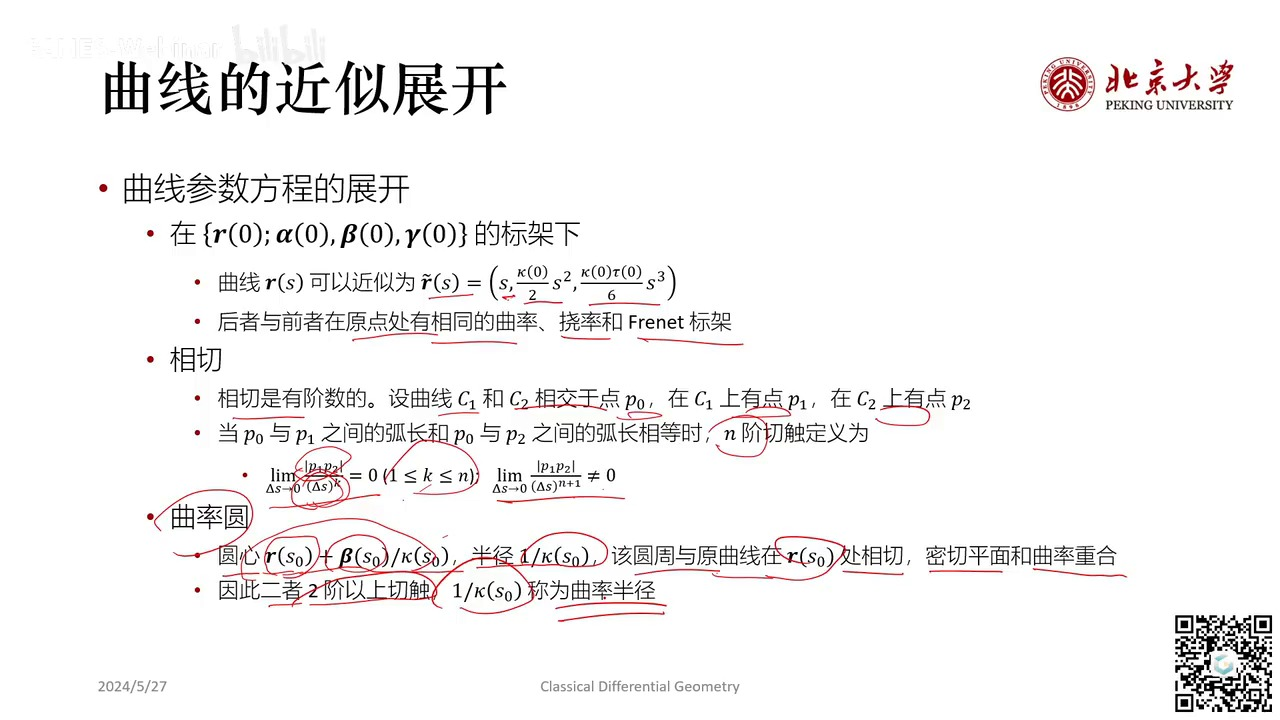
\includegraphics[width=0.92\textwidth]{figures/fig_09_curve_expand.jpg}
\caption{曲线参数方程的近似展开、相切与曲率圆\vtag}
\end{figure}
\srcnote{00:26:15--00:26:30}
\end{minipage}


在 Frenet 标架 $\{\boldsymbol r(0);\boldsymbol\alpha(0),\boldsymbol\beta(0),\boldsymbol\gamma(0)\}$ 下，曲线在原点附近可以近似为
\begin{equation}
\tilde{\boldsymbol r}(s)=\left(s,\ \frac{\kappa(0)}{2}s^2,\ \frac{\kappa(0)\tau(0)}{6}s^3\right).
\end{equation}
后者与前者在原点处有相同的曲率、挠率和 Frenet 标架。

相切是有阶数的。设曲线 $C_1$ 和 $C_2$ 相交于点 $p_0$，在 $C_1$ 上有点 $p_1$，在 $C_2$ 上有点 $p_2$。当 $p_0$ 与 $p_1$ 之间的弧长和 $p_0$ 与 $p_2$ 之间的弧长相等时，$n$ 阶触定义为
\begin{equation}
\lim_{\Delta s\to 0}\frac{|p_1p_2|}{(\Delta s)^k}=0\ (1\le k\le n),\qquad \lim_{\Delta s\to 0}\frac{|p_1p_2|}{(\Delta s)^{n+1}}\ne 0 .
\end{equation}
讲者的解释是：在 $1$ 到 $n$ 次幂上极限都是零，但给它加一次幂就不等于零，这时就说两条曲线 $n$ 阶相切。

曲率圆：圆心为 $\boldsymbol r(s_0)+\boldsymbol\beta(s_0)/\kappa(s_0)$，半径为 $1/\kappa(s_0)$。该圆周与原曲线在 $\boldsymbol r(s_0)$ 处相切，密切平面和曲率都重合，因此二者有 2 阶以上切触。$1/\kappa(s_0)$ 称为曲率半径。

\begin{practicebox}{检验近似展开}
对 $\tilde{\boldsymbol r}(s)$ 直接求导：$\tilde{\boldsymbol r}'(0)=(1,0,0)$，$\tilde{\boldsymbol r}''(0)=(0,\kappa(0),0)$，$\tilde{\boldsymbol r}'''(0)=(0,0,\kappa(0)\tau(0))$。读者可以用一般参数下的曲率与挠率公式验证：原点处曲率为 $\kappa(0)$，挠率为 $\tau(0)$。由此也能看出：曲率决定曲线在密切平面内的“弯”，挠率决定它离开密切平面的“扭”。
\end{practicebox}

\section{参数曲面}

\subsection{定义与正则化}

\noindent\begin{minipage}{\textwidth}
\begin{figure}[H]
\centering
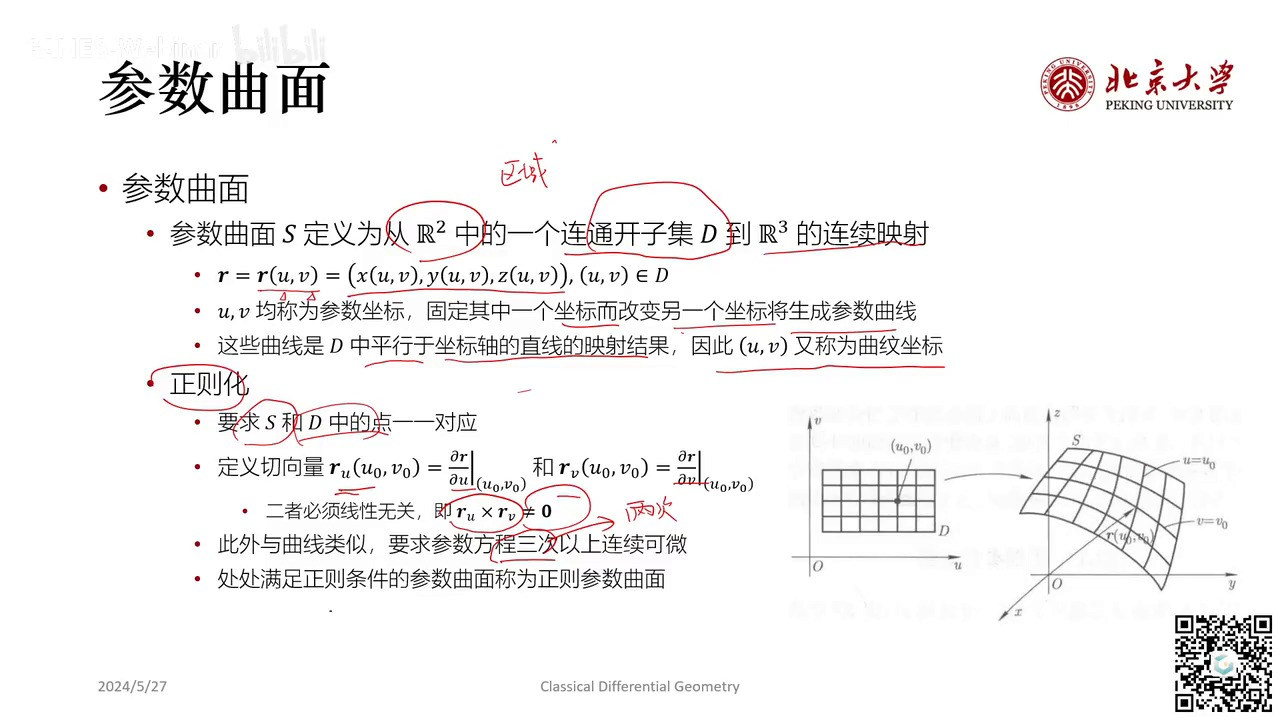
\includegraphics[width=0.92\textwidth]{figures/fig_10_surface.jpg}
\caption{参数曲面的定义与正则化\vtag}
\end{figure}
\srcnote{00:30:00--00:30:15}
\end{minipage}


讲者提到，曲面的参数化与纹理映射密切相关，这部分可以参考 GAMES101 和 GAMES202 中关于纹理映射原理的内容；推荐的参考书是北京大学出版社的《微分几何》。

参数曲面 $S$ 定义为从 $\mathbb R^2$ 中的一个连通开子集 $D$ 到 $\mathbb R^3$ 的连续映射：
\begin{equation}
\boldsymbol r=\boldsymbol r(u,v)=\big(x(u,v),y(u,v),z(u,v)\big),\qquad (u,v)\in D .
\end{equation}
因为定义域是二维的，两个参数坐标分别叫 $u$ 和 $v$。$u,v$ 均称为参数曲线：固定其中一个坐标而改变另一个坐标就生成参数曲线。这些曲线是 $D$ 中平行于坐标轴的直线的映射结果，因此 $(u,v)$ 又称为曲纹坐标。

正则化：要求 $S$ 和 $D$ 中的点一一对应；定义切向量 $\boldsymbol r_u(u_0,v_0)=\frac{\partial\boldsymbol r}{\partial u}\big|_{(u_0,v_0)}$ 和 $\boldsymbol r_v(u_0,v_0)=\frac{\partial\boldsymbol r}{\partial v}\big|_{(u_0,v_0)}$，二者必须线性无关，即 $\boldsymbol r_u\times\boldsymbol r_v\ne\boldsymbol 0$。此外与曲线类似，要求参数方程三次以上连续可微，讲者说实际中往往放宽到两次。处处满足正则条件的参数曲面称为正则参数曲面。

\subsection{正则曲面与参数变换}

\noindent\begin{minipage}{\textwidth}
\begin{figure}[H]
\centering
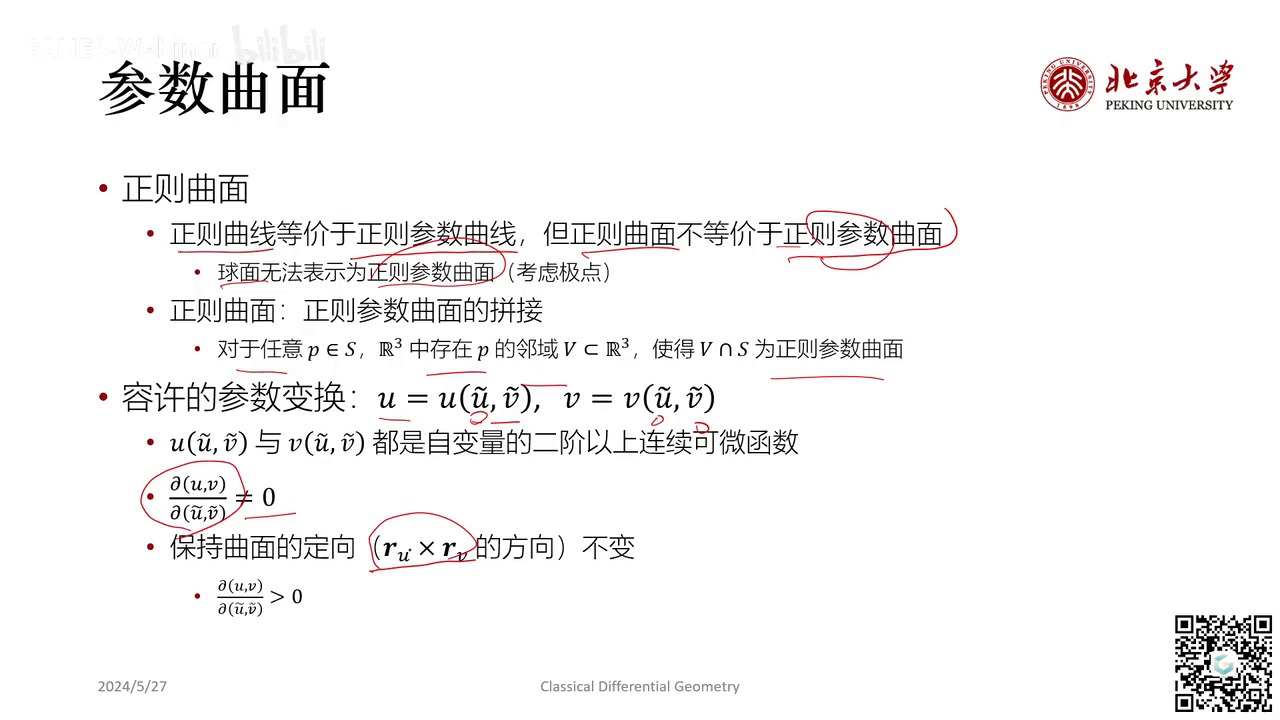
\includegraphics[width=0.92\textwidth]{figures/fig_11_regular_surface.jpg}
\caption{正则曲面与容许的参数变换\vtag}
\end{figure}
\srcnote{00:32:15--00:32:30}
\end{minipage}


正则曲线等价于正则参数曲线，但正则曲面不等价于正则参数曲面。例子是球面：考虑极点，球面无法表示为一个正则参数曲面。正则曲面是正则参数曲面的拼接：对于任意 $p\in S$，$\mathbb R^3$ 中存在 $p$ 的邻域 $V$，使得 $V\cap S$ 为正则参数曲面。讲者解释，球坐标只要不在极点就没有问题，所以只要在极点附近重新做参数化，把那一片变成正则参数曲面，这些正则参数曲面拼在一起就构成了整个球面。

容许的参数变换 $u=u(\tilde u,\tilde v)$，$v=v(\tilde u,\tilde v)$ 需要满足：$u,v$ 都是自变量的二阶以上连续可微函数；$\frac{\partial(u,v)}{\partial(\tilde u,\tilde v)}\ne 0$；若要保持曲面的定向（即 $\boldsymbol r_u\times\boldsymbol r_v$ 的方向）不变，还需 $\frac{\partial(u,v)}{\partial(\tilde u,\tilde v)}>0$。讲者解释，三维空间中的曲面可以决定两个方向，即曲面的正方向和反方向，因为法向量只能朝向其中一侧。

\section{切平面与法线}

\subsection{切向量与切平面}

\noindent\begin{minipage}{\textwidth}
\begin{figure}[H]
\centering
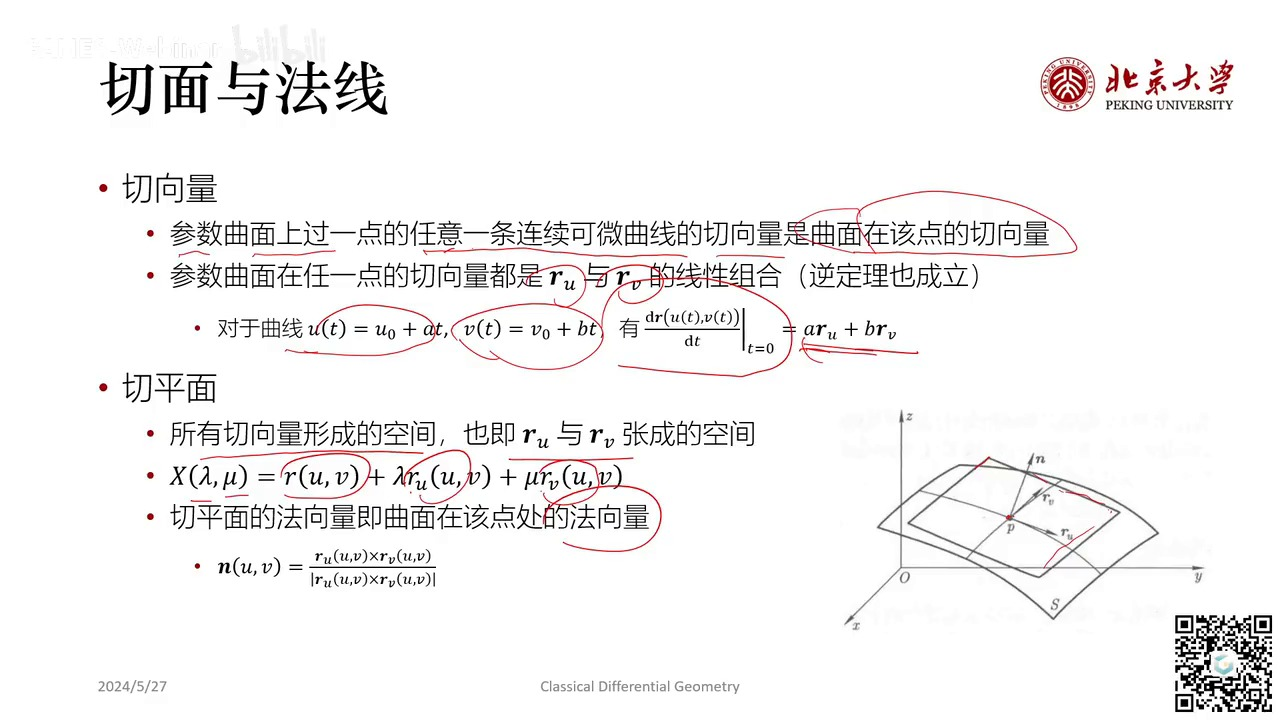
\includegraphics[width=0.92\textwidth]{figures/fig_12_tangent_plane.jpg}
\caption{切向量、切平面与法向量\vtag}
\end{figure}
\srcnote{00:35:00--00:35:15}
\end{minipage}


参数曲面上过一点的任意一条连续可微曲线的切向量，是曲面在该点的切向量。参数曲面在任一点的切向量都是 $\boldsymbol r_u$ 与 $\boldsymbol r_v$ 的线性组合（逆定理也成立）。例如对于曲线 $u(t)=u_0+at$，$v(t)=v_0+bt$，有
\begin{equation}
\left.\frac{\mathrm{d}\boldsymbol r\big(u(t),v(t)\big)}{\mathrm{d}t}\right|_{t=0}=a\boldsymbol r_u+b\boldsymbol r_v .
\end{equation}
所有切向量形成的空间，也即 $\boldsymbol r_u$ 与 $\boldsymbol r_v$ 张成的空间，就是切平面 $\boldsymbol X(\lambda,\mu)=\boldsymbol r(u,v)+\lambda\boldsymbol r_u(u,v)+\mu\boldsymbol r_v(u,v)$。切平面的法向量即曲面在该点处的法向量：
\begin{equation}
\boldsymbol n(u,v)=\frac{\boldsymbol r_u(u,v)\times\boldsymbol r_v(u,v)}{|\boldsymbol r_u(u,v)\times\boldsymbol r_v(u,v)|}.
\end{equation}

\subsection{自然标架与隐式曲面}

与参数曲线类似，$\{\boldsymbol r(u,v);\boldsymbol r_u(u,v),\boldsymbol r_v(u,v),\boldsymbol n(u,v)\}$ 构成了自然标架，后续可以研究自然标架下曲面的性质。

\begin{warningbox}{自然标架一般不是单位正交的}
讲者特别提醒：自然标架中 $\boldsymbol n$ 是单位的，但 $\boldsymbol r_u$、$\boldsymbol r_v$ 一般都不是单位向量；$\boldsymbol n$ 与 $\boldsymbol r_u$、$\boldsymbol r_v$ 都垂直，但 $\boldsymbol r_u$ 与 $\boldsymbol r_v$ 不一定垂直。这和曲线的 Frenet 标架不同，后面的第一基本形正是用来记录这种“不正交、不单位”的度量信息的。
\end{warningbox}

\noindent\begin{minipage}{\textwidth}
\begin{figure}[H]
\centering
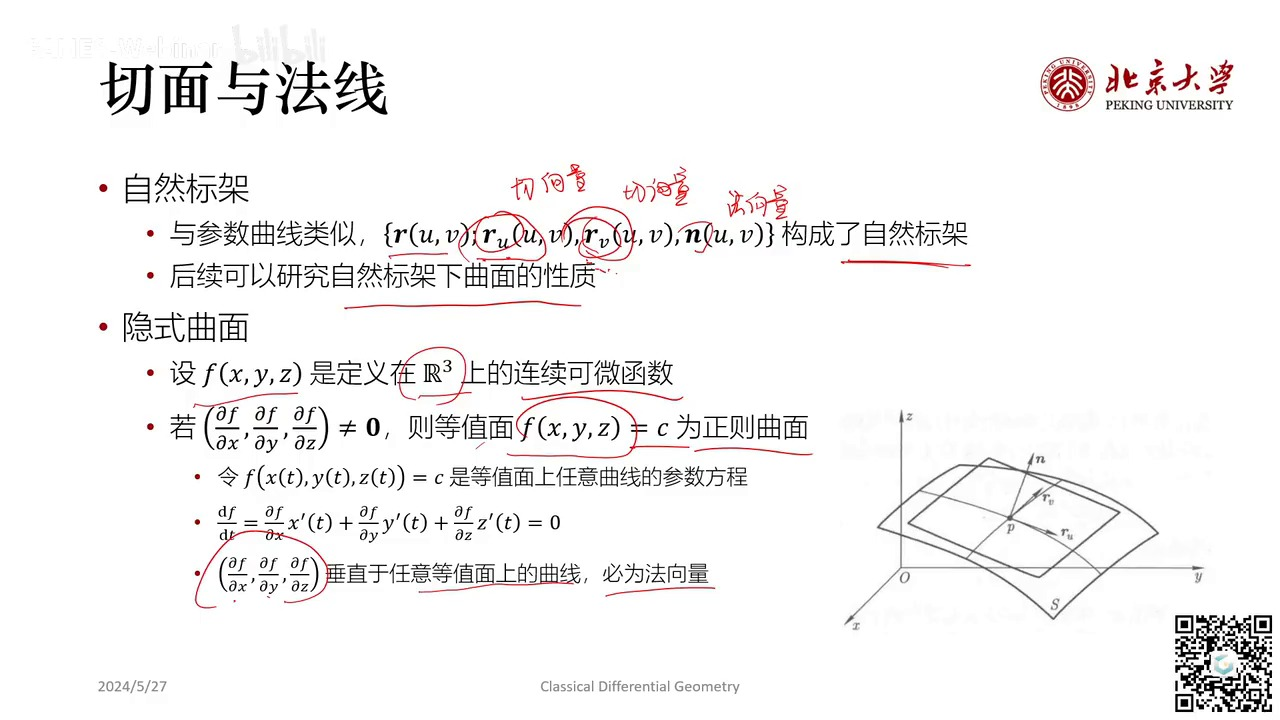
\includegraphics[width=0.92\textwidth]{figures/fig_13_implicit.jpg}
\caption{自然标架与隐式曲面的法向\vtag}
\end{figure}
\srcnote{00:37:00--00:37:15}
\end{minipage}


隐式曲面：设 $f(x,y,z)$ 是定义在 $\mathbb R^3$ 上的连续可微函数。若 $\left(\frac{\partial f}{\partial x},\frac{\partial f}{\partial y},\frac{\partial f}{\partial z}\right)\ne\boldsymbol 0$，则等值面 $f(x,y,z)=c$ 为正则曲面。令 $f\big(x(t),y(t),z(t)\big)=c$ 是等值面上任意曲线的参数方程，对 $t$ 求导得
\begin{equation}
\frac{\partial f}{\partial t}=\frac{\partial f}{\partial x}x'(t)+\frac{\partial f}{\partial y}y'(t)+\frac{\partial f}{\partial z}z'(t)=0 .
\end{equation}
所以梯度 $\nabla f$ 垂直于任意等值面上的曲线，必为法向量。讲者说高等数学上册最后（至少北大版）有隐式曲面的相关内容。

\section{曲面的第一基本形}

\subsection{微线元的长度}

\noindent\begin{minipage}{\textwidth}
\begin{figure}[H]
\centering
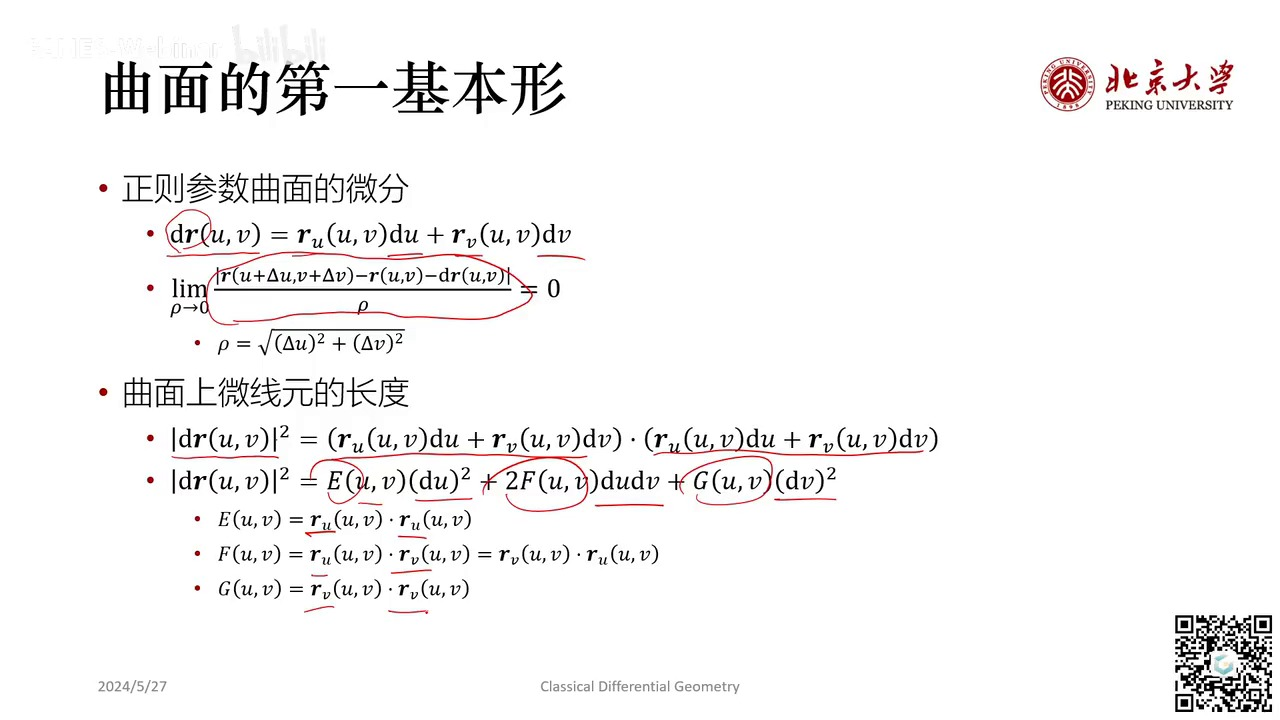
\includegraphics[width=0.92\textwidth]{figures/fig_14_first_form.jpg}
\caption{正则参数曲面的微分与第一基本形\vtag}
\end{figure}
\srcnote{00:38:45--00:39:00}
\end{minipage}


正则参数曲面的微分为 $\mathrm{d}\boldsymbol r(u,v)=\boldsymbol r_u(u,v)\mathrm{d}u+\boldsymbol r_v(u,v)\mathrm{d}v$，意思是
\begin{equation}
\lim_{\rho\to 0}\frac{|\boldsymbol r(u+\Delta u,v+\Delta v)-\boldsymbol r(u,v)-\mathrm{d}\boldsymbol r(u,v)|}{\rho}=0,\qquad \rho=\sqrt{(\Delta u)^2+(\Delta v)^2}.
\end{equation}
$\mathrm{d}\boldsymbol r$ 是线的微元，即线元。考察线元长度的平方：
\begin{equation}
|\mathrm{d}\boldsymbol r(u,v)|^2=E(u,v)(\mathrm{d}u)^2+2F(u,v)\,\mathrm{d}u\,\mathrm{d}v+G(u,v)(\mathrm{d}v)^2,
\end{equation}
其中 $E=\boldsymbol r_u\cdot\boldsymbol r_u$，$F=\boldsymbol r_u\cdot\boldsymbol r_v=\boldsymbol r_v\cdot\boldsymbol r_u$，$G=\boldsymbol r_v\cdot\boldsymbol r_v$。

\subsection{第一基本形}

\noindent\begin{minipage}{\textwidth}
\begin{figure}[H]
\centering
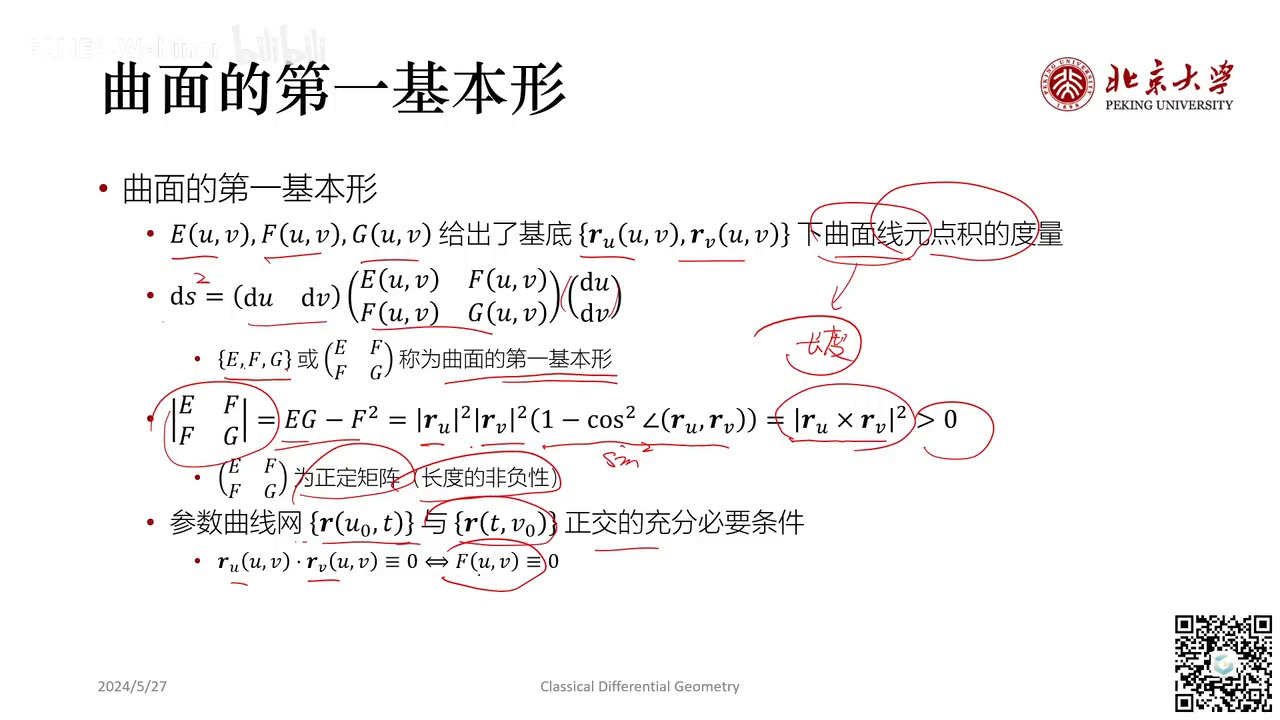
\includegraphics[width=0.92\textwidth]{figures/fig_15_first_form_matrix.jpg}
\caption{第一基本形的矩阵形式及其正定性\vtag}
\end{figure}
\srcnote{00:41:00--00:41:15}
\end{minipage}


$E(u,v),F(u,v),G(u,v)$ 三个标量函数给出了基底 $\{\boldsymbol r_u,\boldsymbol r_v\}$ 下曲面线元点积的度量。写成矩阵形式
\begin{equation}
\mathrm{d}s^2=\begin{pmatrix}\mathrm{d}u&\mathrm{d}v\end{pmatrix}\begin{pmatrix}E&F\\F&G\end{pmatrix}\begin{pmatrix}\mathrm{d}u\\ \mathrm{d}v\end{pmatrix},
\end{equation}
$\{E,F,G\}$ 或矩阵 $\begin{pmatrix}E&F\\F&G\end{pmatrix}$ 称为曲面的第一基本形。对它求行列式：
\begin{equation}
\begin{vmatrix}E&F\\F&G\end{vmatrix}=EG-F^2=|\boldsymbol r_u|^2|\boldsymbol r_v|^2\big(1-\cos^2\angle(\boldsymbol r_u,\boldsymbol r_v)\big)=|\boldsymbol r_u\times\boldsymbol r_v|^2>0,
\end{equation}
所以第一基本形是正定矩阵，这也保证了长度的非负性。

参数曲线网 $\{\boldsymbol r(u_0,t)\}$ 与 $\{\boldsymbol r(t,v_0)\}$ 正交的充分必要条件是 $\boldsymbol r_u(u,v)\cdot\boldsymbol r_v(u,v)\equiv 0$，即 $F(u,v)\equiv 0$。

\subsection{曲面上的弧长与面积}

\noindent\begin{minipage}{\textwidth}
\begin{figure}[H]
\centering
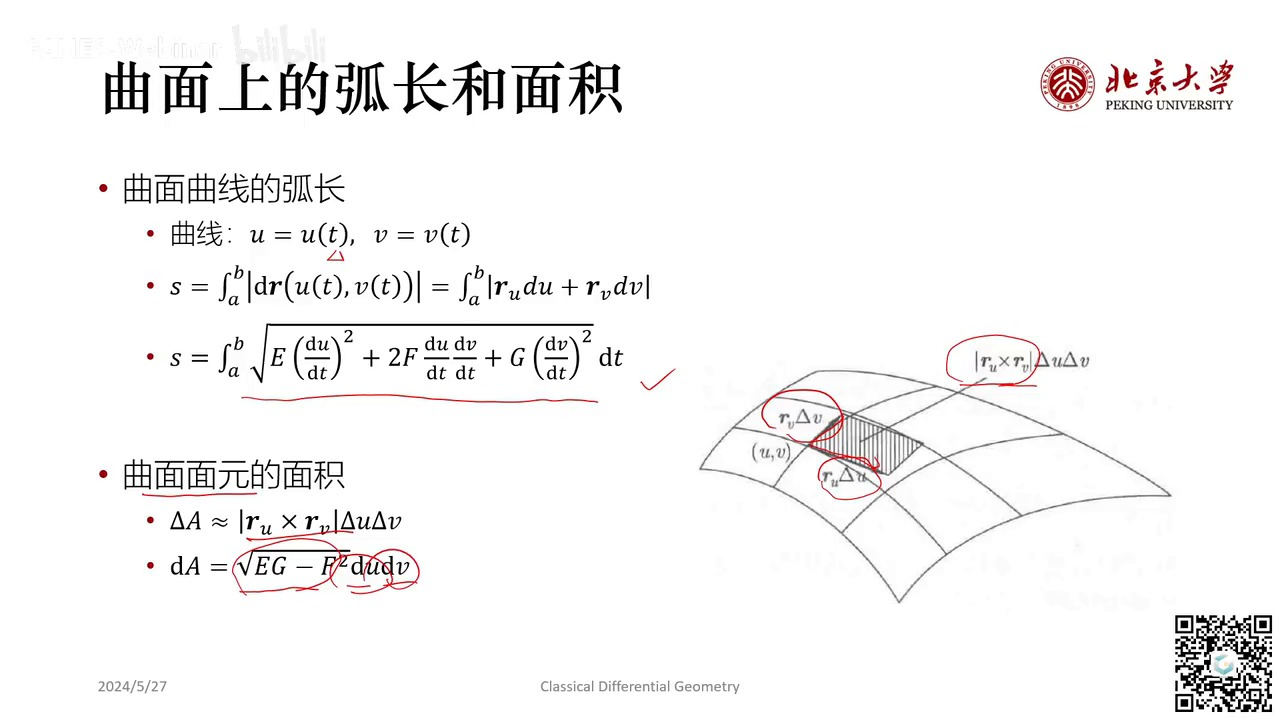
\includegraphics[width=0.92\textwidth]{figures/fig_16_area.jpg}
\caption{曲面曲线的弧长与曲面面元的面积\vtag}
\end{figure}
\srcnote{00:42:45--00:43:00}
\end{minipage}


曲面上的曲线 $u=u(t)$，$v=v(t)$ 的弧长为
\begin{equation}
s=\int_a^b\left|\mathrm{d}\boldsymbol r\big(u(t),v(t)\big)\right|=\int_a^b\sqrt{E\left(\frac{\mathrm{d}u}{\mathrm{d}t}\right)^2+2F\frac{\mathrm{d}u}{\mathrm{d}t}\frac{\mathrm{d}v}{\mathrm{d}t}+G\left(\frac{\mathrm{d}v}{\mathrm{d}t}\right)^2}\,\mathrm{d}t .
\end{equation}
曲面面元的面积：沿 $u$ 方向走一截得到 $\boldsymbol r_u\Delta u$，沿 $v$ 方向走一截得到 $\boldsymbol r_v\Delta v$，二者张成的平行四边形面积为 $\Delta A\approx|\boldsymbol r_u\times\boldsymbol r_v|\Delta u\Delta v$，于是
\begin{equation}
\mathrm{d}A=\sqrt{EG-F^2}\,\mathrm{d}u\,\mathrm{d}v .
\end{equation}

\section{保长、保角与可展曲面}

\subsection{保长变换}

\noindent\begin{minipage}{\textwidth}
\begin{figure}[H]
\centering
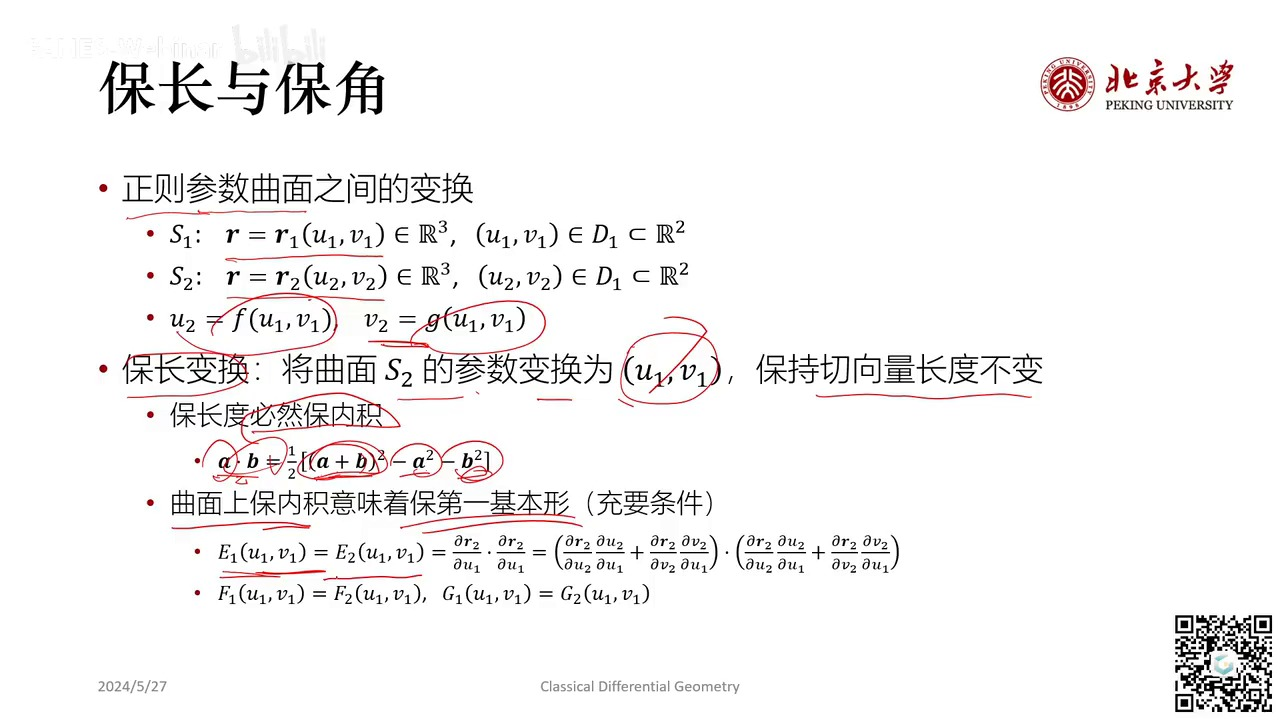
\includegraphics[width=0.92\textwidth]{figures/fig_17_isometry.jpg}
\caption{正则参数曲面之间的变换与保长变换\vtag}
\end{figure}
\srcnote{00:44:45--00:45:00}
\end{minipage}


正则参数曲面往往对应好多种不同的参数化方法，这就引出了保长与保角。考虑正则参数曲面之间的变换：$S_1:\boldsymbol r=\boldsymbol r_1(u_1,v_1)$，$S_2:\boldsymbol r=\boldsymbol r_2(u_2,v_2)$，$u_2=f(u_1,v_1)$，$v_2=g(u_1,v_1)$。

保长变换是说：将曲面 $S_2$ 的参数变换为 $(u_1,v_1)$，保持切向量长度不变。保长度必然保内积，因为内积可以写成长度的组合：
\begin{equation}
\boldsymbol a\cdot\boldsymbol b=\frac{1}{2}\left[(\boldsymbol a+\boldsymbol b)^2-\boldsymbol a^2-\boldsymbol b^2\right].
\end{equation}
所以曲面上保内积意味着保第一基本形，这是充要条件：$E_1(u_1,v_1)=E_2(u_1,v_1)$，$F_1=F_2$，$G_1=G_2$。

\subsection{保角变换}

\noindent\begin{minipage}{\textwidth}
\begin{figure}[H]
\centering
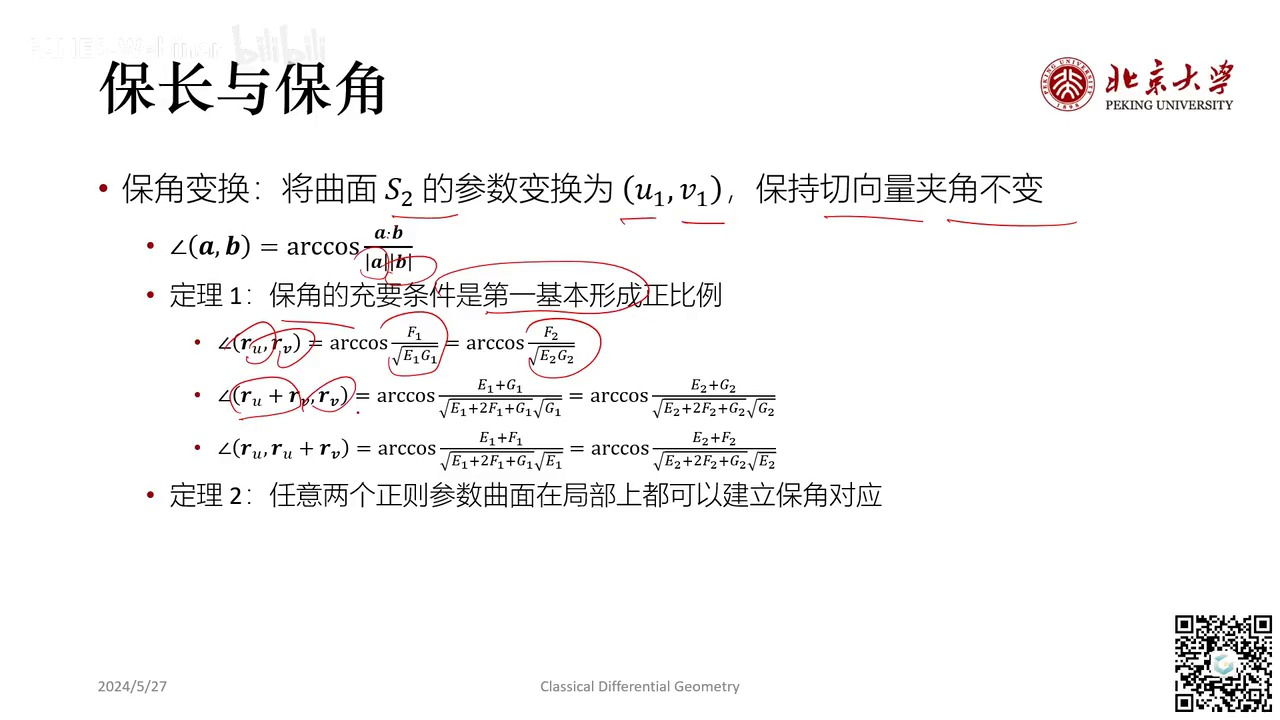
\includegraphics[width=0.92\textwidth]{figures/fig_18_conformal.jpg}
\caption{保角变换的充要条件：第一基本形成正比例\vtag}
\end{figure}
\srcnote{00:46:00--00:46:15}
\end{minipage}


保角变换是说：将曲面 $S_2$ 的参数变换为 $(u_1,v_1)$，保持切向量夹角不变，夹角为 $\angle(\boldsymbol a,\boldsymbol b)=\arccos\frac{\boldsymbol a\cdot\boldsymbol b}{|\boldsymbol a||\boldsymbol b|}$。

定理一：保角的充要条件是第一基本形成正比例。分别取 $\boldsymbol r_u$ 与 $\boldsymbol r_v$、$\boldsymbol r_u+\boldsymbol r_v$ 与 $\boldsymbol r_v$、$\boldsymbol r_u+\boldsymbol r_v$ 与 $\boldsymbol r_u$ 这几对切向量，写出它们的夹角相等的恒等式，例如
\begin{equation}
\arccos\frac{F_1}{\sqrt{E_1G_1}}=\arccos\frac{F_2}{\sqrt{E_2G_2}},
\end{equation}
联立即可推出 $E_1:F_1:G_1=E_2:F_2:G_2$。定理二：任意两个正则参数曲面在局部上都可以建立保角对应。

\noindent\begin{minipage}{\textwidth}
\begin{figure}[H]
\centering
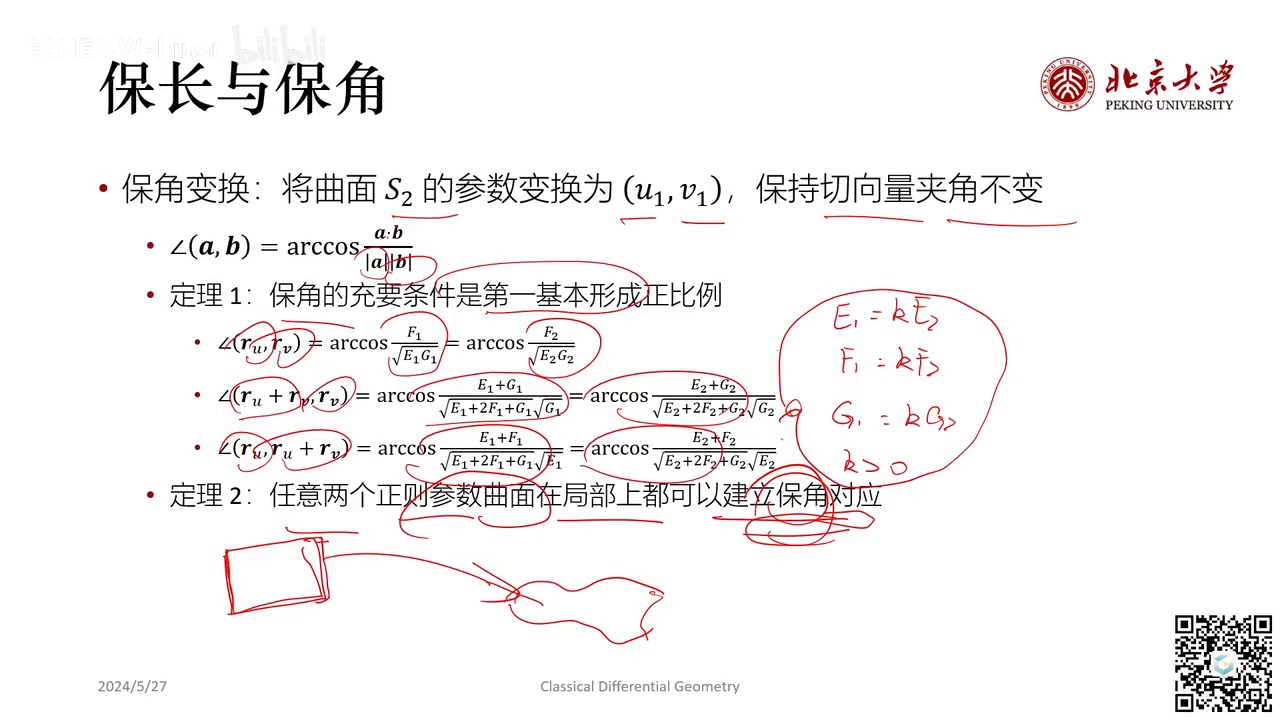
\includegraphics[width=0.92\textwidth]{figures/fig_19_conformal_note.jpg}
\caption{讲者在保角定理旁列出的比例关系\vtag}
\end{figure}
\srcnote{00:47:45--00:48:00}
\end{minipage}


\begin{importantbox}{为什么图形学关心保长和保角}
讲者联系了纹理映射：纹理是一张张平面上的贴图，而要映射到的是三维曲面。我们希望映射过来之后不要丢失太多信息，尤其希望存储时参数化尽量均匀。保长的映射最理想，但一般不存在（球面就不能保长地展平）；退而求其次，保角映射总是局部存在的，它保持小图案的形状，只改变大小。这正是曲面参数化算法中“共形参数化”的理论来源（后一句由讲义作者补充）。
\end{importantbox}

\subsection{直纹面与可展曲面}

\noindent\begin{minipage}{\textwidth}
\begin{figure}[H]
\centering
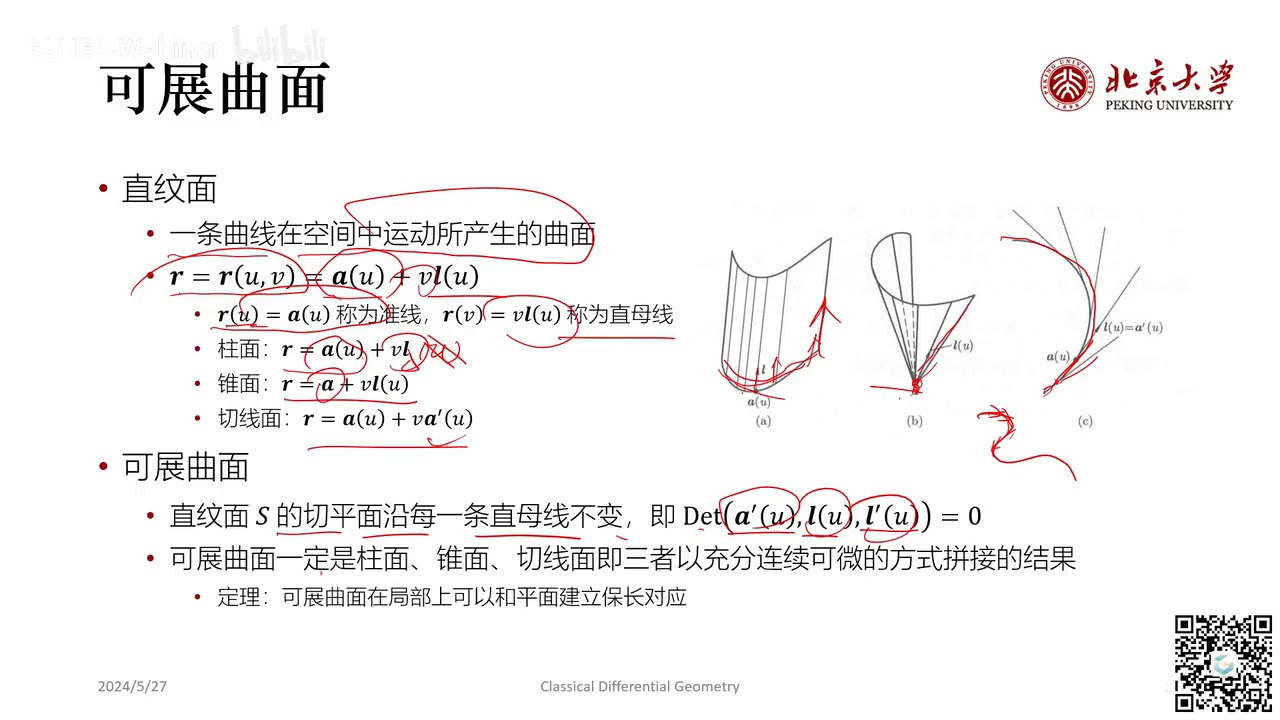
\includegraphics[width=0.92\textwidth]{figures/fig_20_developable.jpg}
\caption{直纹面（柱面、锥面、切线面）与可展曲面\vtag}
\end{figure}
\srcnote{00:50:30--00:50:45}
\end{minipage}


什么叫可展曲面？先看直纹面：一条直线在空间中运动所产生的曲面，称为直纹面，
\begin{equation}
\boldsymbol r=\boldsymbol r(u,v)=\boldsymbol a(u)+v\boldsymbol l(u).
\end{equation}
$\boldsymbol r(u)=\boldsymbol a(u)$ 称为准线，$\boldsymbol r(v)=v\boldsymbol l(u)$ 称为直母线。若方向 $\boldsymbol l$ 始终是定值，得到柱面 $\boldsymbol r=\boldsymbol a(u)+v\boldsymbol l$；若准线 $\boldsymbol a$ 是定点，得到锥面 $\boldsymbol r=\boldsymbol a+v\boldsymbol l(u)$；若直母线取准线的切线，得到切线面 $\boldsymbol r=\boldsymbol a(u)+v\boldsymbol a'(u)$。

可展曲面：直纹面 $S$ 的切平面沿每一条直母线不变，即 $\det\big(\boldsymbol a'(u),\boldsymbol l(u),\boldsymbol l'(u)\big)=0$。可展曲面一定是柱面、锥面、切线面这三者以充分连续可微的方式拼接的结果。定理：可展曲面在局部上可以和平面建立保长对应。

\begin{knowledgebox}{布料与可展曲面}
讲者的例子：想象一块处处不可拉伸的布料。所谓不可拉伸，是说布料上任意两个点，当布料被揉成一团以后，沿着曲面去看这两点之间的距离是不变的。这块布放平的时候是平面，运动之后揉成什么形状，那个形状都必须与平面保长对应，也就是可展曲面。这一点在布料模拟中很有用。
\end{knowledgebox}

\section{曲面的第二基本形}

\subsection{定义}

\noindent\begin{minipage}{\textwidth}
\begin{figure}[H]
\centering
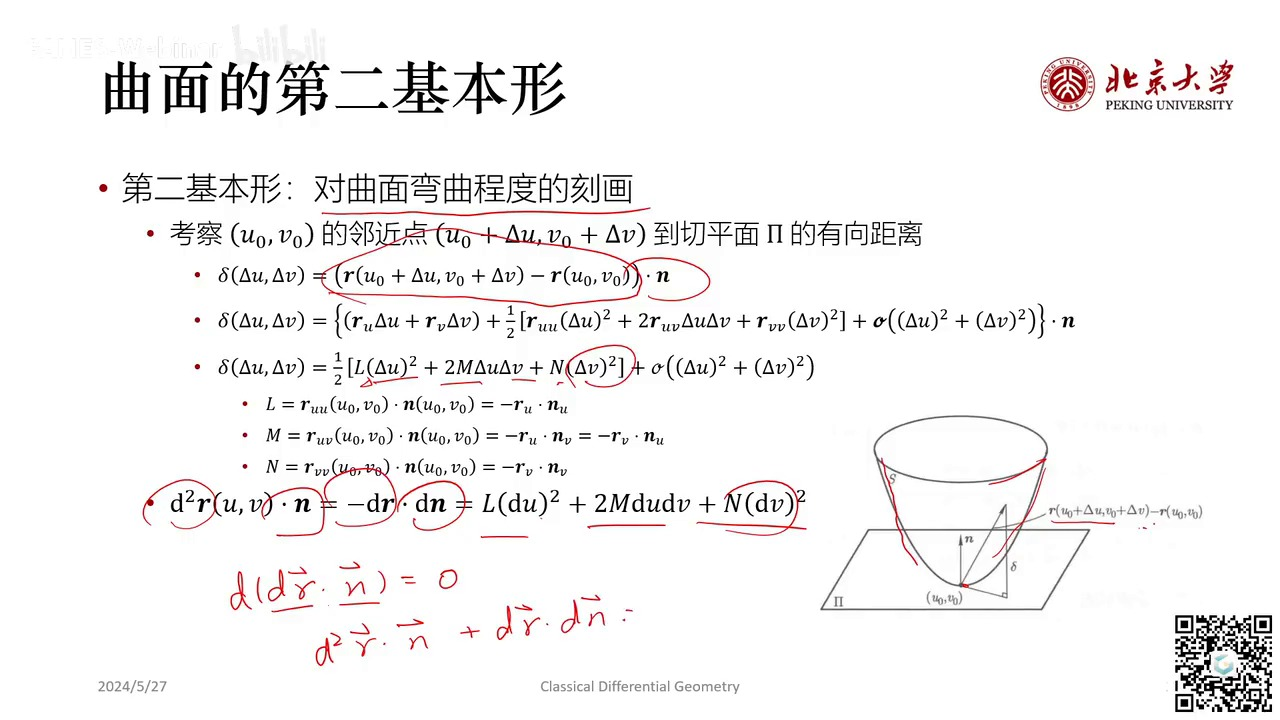
\includegraphics[width=0.92\textwidth]{figures/fig_21_second_form.jpg}
\caption{第二基本形：邻近点到切平面的有向距离\vtag}
\end{figure}
\srcnote{00:54:15--00:54:30}
\end{minipage}


曲面有了第一基本形，必然还会有第二基本形。第二基本形是对曲面弯曲程度的刻画。考察 $(u_0,v_0)$ 的邻近点 $(u_0+\Delta u,v_0+\Delta v)$ 到切平面 $\Pi$ 的有向距离：
\begin{equation}
\delta(\Delta u,\Delta v)=\big(\boldsymbol r(u_0+\Delta u,v_0+\Delta v)-\boldsymbol r(u_0,v_0)\big)\cdot\boldsymbol n .
\end{equation}
做二阶泰勒展开，一阶项 $\boldsymbol r_u\Delta u+\boldsymbol r_v\Delta v$ 在切平面内，与法向点乘为零，只剩二阶项：
\begin{equation}
\delta(\Delta u,\Delta v)=\frac{1}{2}\left[L(\Delta u)^2+2M\Delta u\Delta v+N(\Delta v)^2\right]+o\big((\Delta u)^2+(\Delta v)^2\big),
\end{equation}
其中 $L=\boldsymbol r_{uu}\cdot\boldsymbol n=-\boldsymbol r_u\cdot\boldsymbol n_u$，$M=\boldsymbol r_{uv}\cdot\boldsymbol n=-\boldsymbol r_u\cdot\boldsymbol n_v=-\boldsymbol r_v\cdot\boldsymbol n_u$，$N=\boldsymbol r_{vv}\cdot\boldsymbol n=-\boldsymbol r_v\cdot\boldsymbol n_v$。等价地，
\begin{equation}
\mathrm{d}^2\boldsymbol r(u,v)\cdot\boldsymbol n=-\mathrm{d}\boldsymbol r\cdot\mathrm{d}\boldsymbol n=L(\mathrm{d}u)^2+2M\,\mathrm{d}u\,\mathrm{d}v+N(\mathrm{d}v)^2 .
\end{equation}
讲者解释第二个等号：因为 $\mathrm{d}\boldsymbol r\cdot\boldsymbol n\equiv 0$，对它再取一次微分即得 $\mathrm{d}^2\boldsymbol r\cdot\boldsymbol n+\mathrm{d}\boldsymbol r\cdot\mathrm{d}\boldsymbol n=0$。

\subsection{平面和球面的第二基本形}

\noindent\begin{minipage}{\textwidth}
\begin{figure}[H]
\centering
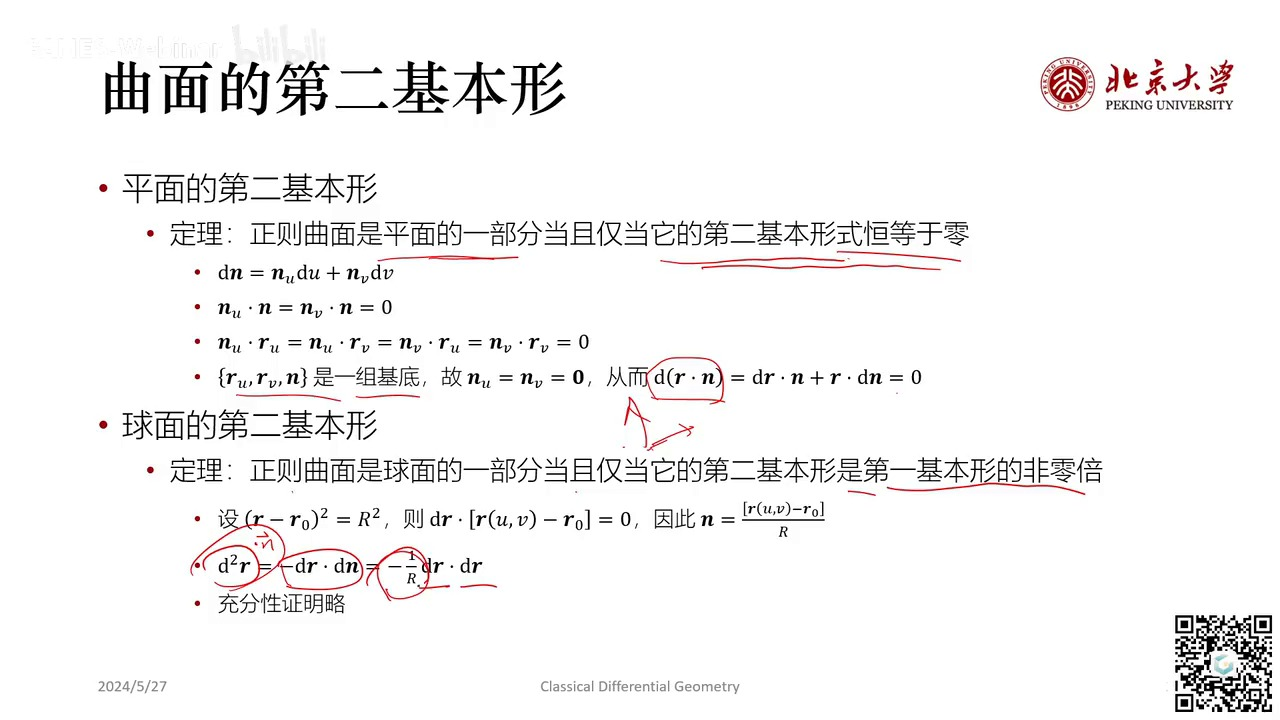
\includegraphics[width=0.92\textwidth]{figures/fig_22_second_form_examples.jpg}
\caption{平面与球面的第二基本形\vtag}
\end{figure}
\srcnote{00:56:45--00:57:00}
\end{minipage}


第二基本形有什么用？先看两个特殊曲面。定理：正则曲面是平面的一部分，当且仅当它的第二基本形式恒等于零。证明：$\mathrm{d}\boldsymbol n=\boldsymbol n_u\mathrm{d}u+\boldsymbol n_v\mathrm{d}v$；由 $\boldsymbol n\cdot\boldsymbol n=1$ 得 $\boldsymbol n_u\cdot\boldsymbol n=\boldsymbol n_v\cdot\boldsymbol n=0$；第二基本形为零又给出 $\boldsymbol n_u\cdot\boldsymbol r_u=\boldsymbol n_u\cdot\boldsymbol r_v=\boldsymbol n_v\cdot\boldsymbol r_u=\boldsymbol n_v\cdot\boldsymbol r_v=0$。而 $\{\boldsymbol r_u,\boldsymbol r_v,\boldsymbol n\}$ 是一组基底，故 $\boldsymbol n_u=\boldsymbol n_v=\boldsymbol 0$，从而 $\mathrm{d}(\boldsymbol r\cdot\boldsymbol n)=\mathrm{d}\boldsymbol r\cdot\boldsymbol n+\boldsymbol r\cdot\mathrm{d}\boldsymbol n=0$，曲面在一个平面内。

定理：正则曲面是球面的一部分，当且仅当它的第二基本形是第一基本形的非零倍。设 $(\boldsymbol r-\boldsymbol r_0)^2=R^2$，则 $\mathrm{d}\boldsymbol r\cdot[\boldsymbol r(u,v)-\boldsymbol r_0]=0$，因此法向量 $\boldsymbol n=\frac{\boldsymbol r(u,v)-\boldsymbol r_0}{R}$，于是 $\mathrm{d}^2\boldsymbol r\cdot\boldsymbol n=-\mathrm{d}\boldsymbol r\cdot\mathrm{d}\boldsymbol n=-\frac{1}{R}\mathrm{d}\boldsymbol r\cdot\mathrm{d}\boldsymbol r$。充分性证明从略。

\section{曲面的曲率}

\subsection{法曲率与梅尼埃定理}

\noindent\begin{minipage}{\textwidth}
\begin{figure}[H]
\centering
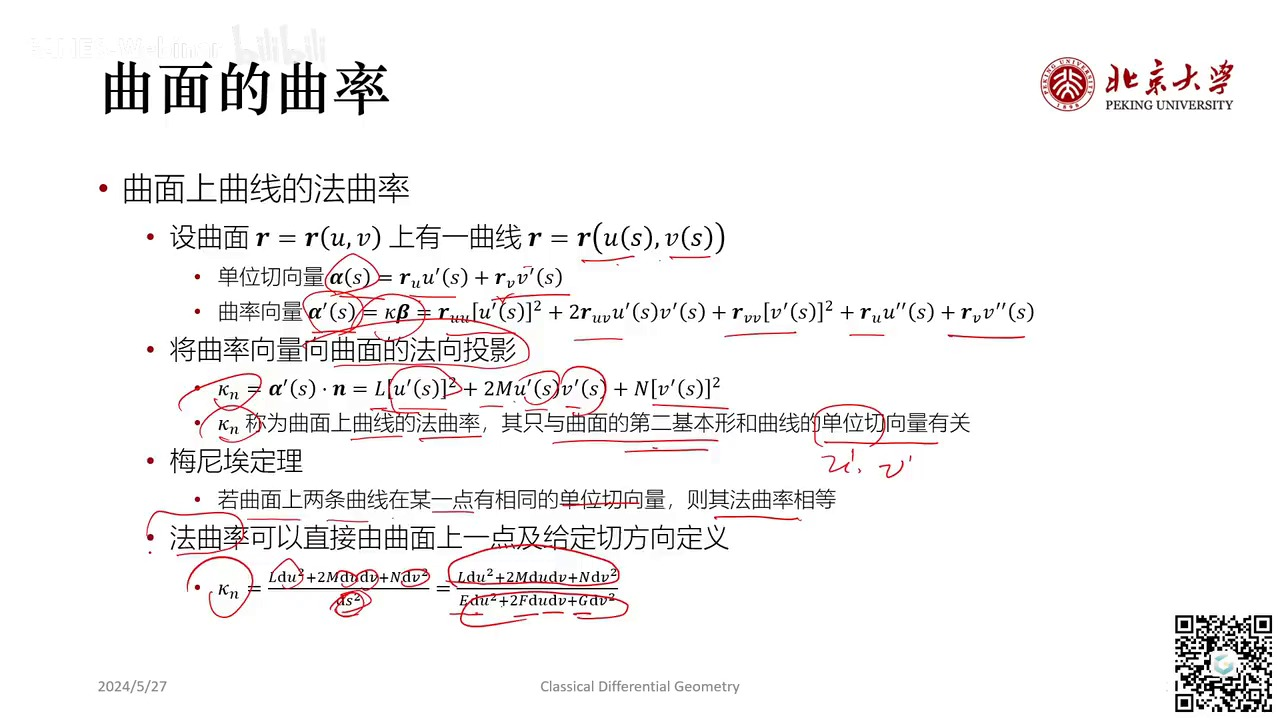
\includegraphics[width=0.92\textwidth]{figures/fig_23_normal_curvature.jpg}
\caption{曲面上曲线的法曲率与梅尼埃定理\vtag}
\end{figure}
\srcnote{00:59:30--00:59:45}
\end{minipage}


设曲面 $\boldsymbol r=\boldsymbol r(u,v)$ 上有一曲线 $\boldsymbol r=\boldsymbol r\big(u(s),v(s)\big)$，$s$ 为弧长。单位切向量 $\boldsymbol\alpha(s)=\boldsymbol r_uu'(s)+\boldsymbol r_vv'(s)$，曲率向量
\begin{equation}
\boldsymbol\alpha'(s)=\kappa\boldsymbol\beta=\boldsymbol r_{uu}[u'(s)]^2+2\boldsymbol r_{uv}u'(s)v'(s)+\boldsymbol r_{vv}[v'(s)]^2+\boldsymbol r_uu''(s)+\boldsymbol r_vv''(s).
\end{equation}
将曲率向量向曲面的法向投影，$\boldsymbol r_u$、$\boldsymbol r_v$ 两项与法向垂直而消失：
\begin{equation}
\kappa_n=\boldsymbol\alpha'(s)\cdot\boldsymbol n=L[u'(s)]^2+2Mu'(s)v'(s)+N[v'(s)]^2 .
\end{equation}
$\kappa_n$ 称为曲面上曲线的法曲率，它只与曲面的第二基本形和曲线的单位切向量有关。由此得到梅尼埃定理：若曲面上两条曲线在某一点有相同的单位切向量，则其法曲率相等。所以法曲率可以直接由曲面上一点及给定切方向定义，因为 $u'=\mathrm{d}u/\mathrm{d}s$，$\mathrm{d}s^2$ 又由第一基本形给出：
\begin{equation}
\kappa_n=\frac{L\,\mathrm{d}u^2+2M\,\mathrm{d}u\,\mathrm{d}v+N\,\mathrm{d}v^2}{\mathrm{d}s^2}=\frac{L\,\mathrm{d}u^2+2M\,\mathrm{d}u\,\mathrm{d}v+N\,\mathrm{d}v^2}{E\,\mathrm{d}u^2+2F\,\mathrm{d}u\,\mathrm{d}v+G\,\mathrm{d}v^2}.
\end{equation}
讲者说，这样就可以抛开具体的那条曲线，直接这样定义法曲率。

\subsection{法截线与欧拉公式}

\noindent\begin{minipage}{\textwidth}
\begin{figure}[H]
\centering
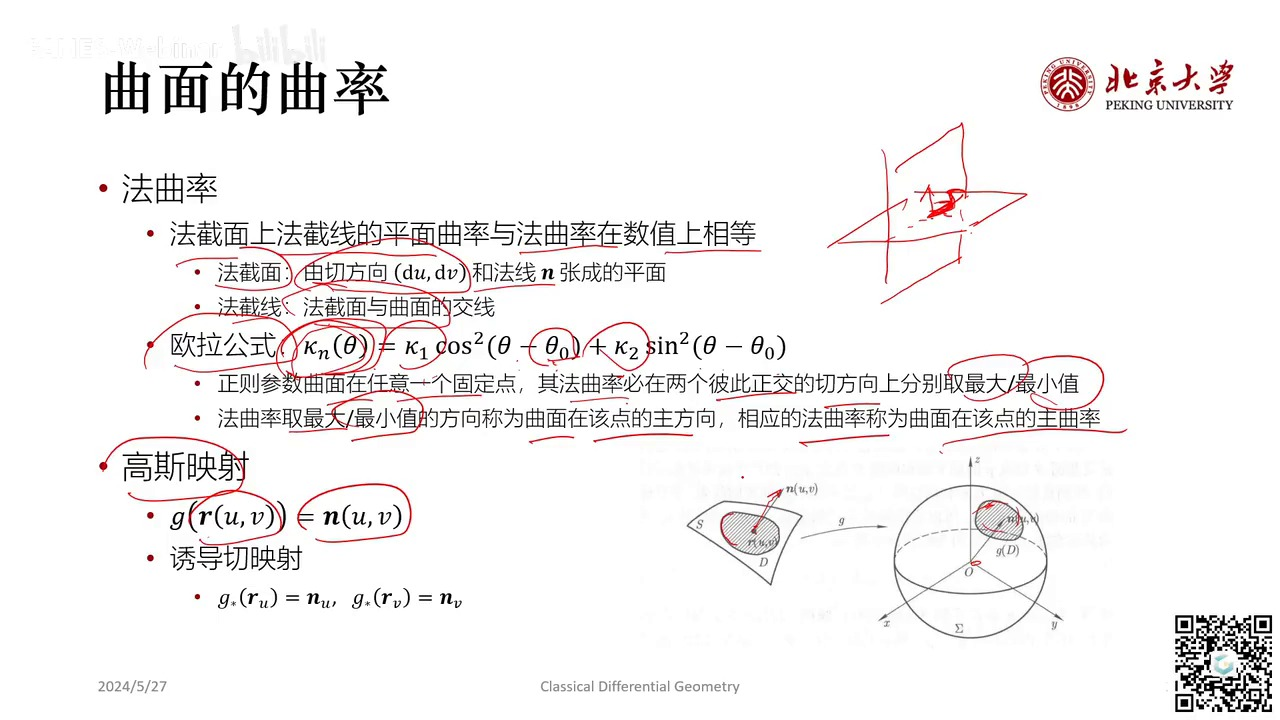
\includegraphics[width=0.92\textwidth]{figures/fig_24_euler.jpg}
\caption{法截线、欧拉公式与高斯映射\vtag}
\end{figure}
\srcnote{01:02:45--01:03:00}
\end{minipage}


法截面上法截线的平面曲率，与法曲率在数值上相等。法截面是由切方向 $(\mathrm{d}u,\mathrm{d}v)$ 和法线 $\boldsymbol n$ 张成的平面，法截线是法截面与曲面的交线。欧拉公式：
\begin{equation}
\kappa_n(\theta)=\kappa_1\cos^2(\theta-\theta_0)+\kappa_2\sin^2(\theta-\theta_0).
\end{equation}
它说明正则参数曲面在任意一个固定点，其法曲率必在两个彼此正交的切方向上分别取最大值和最小值。法曲率取最大值、最小值的方向称为曲面在该点的主方向，相应的法曲率称为曲面在该点的主曲率。

\subsection{高斯映射与魏因加滕映射}

怎么证明欧拉公式？讲者说有一种漂亮的方法，但需要多一点数学。考察高斯映射：它把曲面上的点映射为该点的单位法向量，$g\big(\boldsymbol r(u,v)\big)=\boldsymbol n(u,v)$，即把法向量平移到单位球面上。由高斯映射可以得到诱导的切映射 $g_*$：$g_*(\boldsymbol r_u)=\boldsymbol n_u$，$g_*(\boldsymbol r_v)=\boldsymbol n_v$。

\noindent\begin{minipage}{\textwidth}
\begin{figure}[H]
\centering
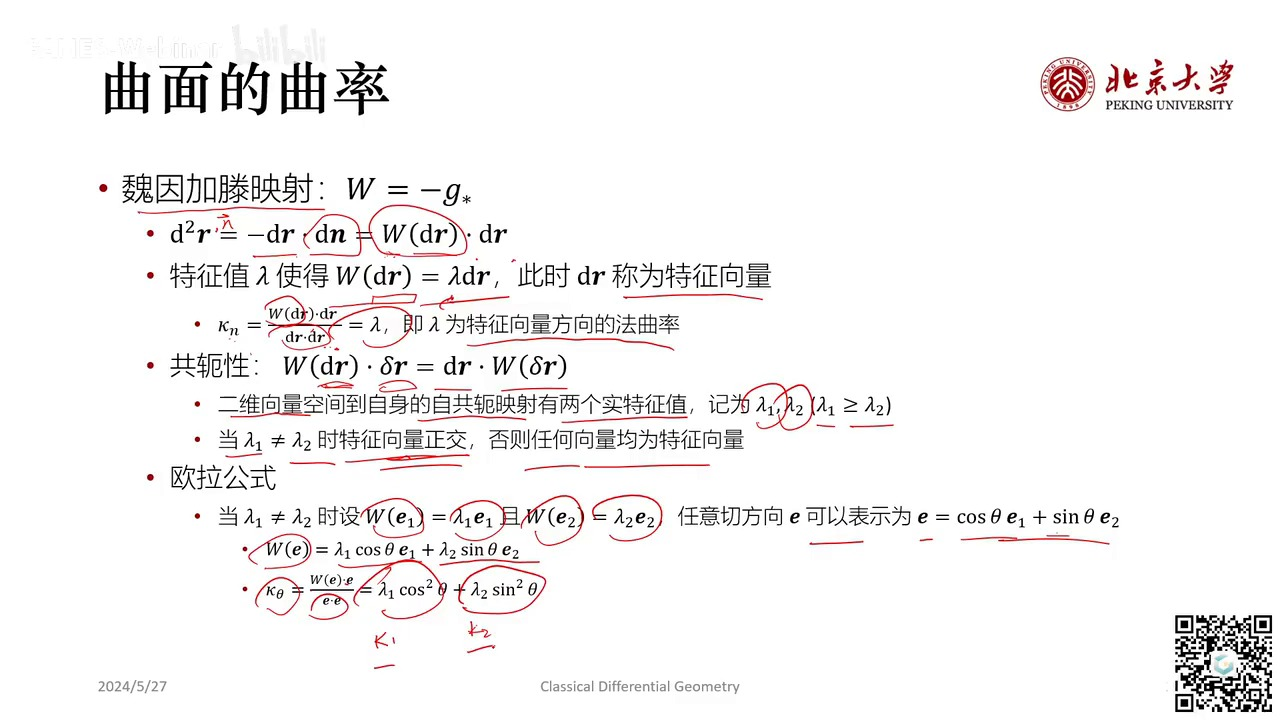
\includegraphics[width=0.92\textwidth]{figures/fig_25_weingarten.jpg}
\caption{魏因加滕映射、共轭性与欧拉公式的证明\vtag}
\end{figure}
\srcnote{01:06:45--01:07:00}
\end{minipage}


记魏因加滕（Weingarten）映射 $W=-g_*$，于是第二基本形可写成 $\mathrm{d}^2\boldsymbol r\cdot\boldsymbol n=-\mathrm{d}\boldsymbol r\cdot\mathrm{d}\boldsymbol n=W(\mathrm{d}\boldsymbol r)\cdot\mathrm{d}\boldsymbol r$。$W$ 是线性映射。若存在特征值 $\lambda$ 使得 $W(\mathrm{d}\boldsymbol r)=\lambda\,\mathrm{d}\boldsymbol r$，此时 $\mathrm{d}\boldsymbol r$ 称为特征向量，并且
\begin{equation}
\kappa_n=\frac{W(\mathrm{d}\boldsymbol r)\cdot\mathrm{d}\boldsymbol r}{\mathrm{d}\boldsymbol r\cdot\mathrm{d}\boldsymbol r}=\lambda,
\end{equation}
即 $\lambda$ 为特征向量方向的法曲率。

$W$ 具有共轭性：任取两个切向量 $\mathrm{d}\boldsymbol r$ 和 $\delta\boldsymbol r$，有 $W(\mathrm{d}\boldsymbol r)\cdot\delta\boldsymbol r=\mathrm{d}\boldsymbol r\cdot W(\delta\boldsymbol r)$，也就是说它是自伴的。二维向量空间到自身的自共轭映射有两个实特征值，记为 $\lambda_1,\lambda_2$（$\lambda_1\ge\lambda_2$）；当 $\lambda_1\ne\lambda_2$ 时特征向量正交，否则任何向量均为特征向量。

欧拉公式的证明：当 $\lambda_1\ne\lambda_2$ 时，设 $W(\boldsymbol e_1)=\lambda_1\boldsymbol e_1$ 且 $W(\boldsymbol e_2)=\lambda_2\boldsymbol e_2$，任意切方向 $\boldsymbol e$ 可以表示为 $\boldsymbol e=\cos\theta\,\boldsymbol e_1+\sin\theta\,\boldsymbol e_2$，于是
\begin{equation}
W(\boldsymbol e)=\lambda_1\cos\theta\,\boldsymbol e_1+\lambda_2\sin\theta\,\boldsymbol e_2,\qquad \kappa_n=\frac{W(\boldsymbol e)\cdot\boldsymbol e}{\boldsymbol e\cdot\boldsymbol e}=\lambda_1\cos^2\theta+\lambda_2\sin^2\theta .
\end{equation}

\begin{knowledgebox}{这就是第三讲的特征值问题}
讲义作者补充：魏因加滕映射在基底 $\{\boldsymbol r_u,\boldsymbol r_v\}$ 下的矩阵就是 $\mathrm{I}^{-1}\mathrm{II}$，其中 $\mathrm{I}=\begin{pmatrix}E&F\\F&G\end{pmatrix}$，$\mathrm{II}=\begin{pmatrix}L&M\\M&N\end{pmatrix}$。主曲率就是这个矩阵的特征值，主方向就是特征向量；欧拉公式不过是对称矩阵在特征基下的瑞利商。离散网格上估计曲率时，也是先估计这个“形状算子”，再做特征分解。
\end{knowledgebox}

\subsection{脐点、平均曲率与高斯曲率}

\noindent\begin{minipage}{\textwidth}
\begin{figure}[H]
\centering
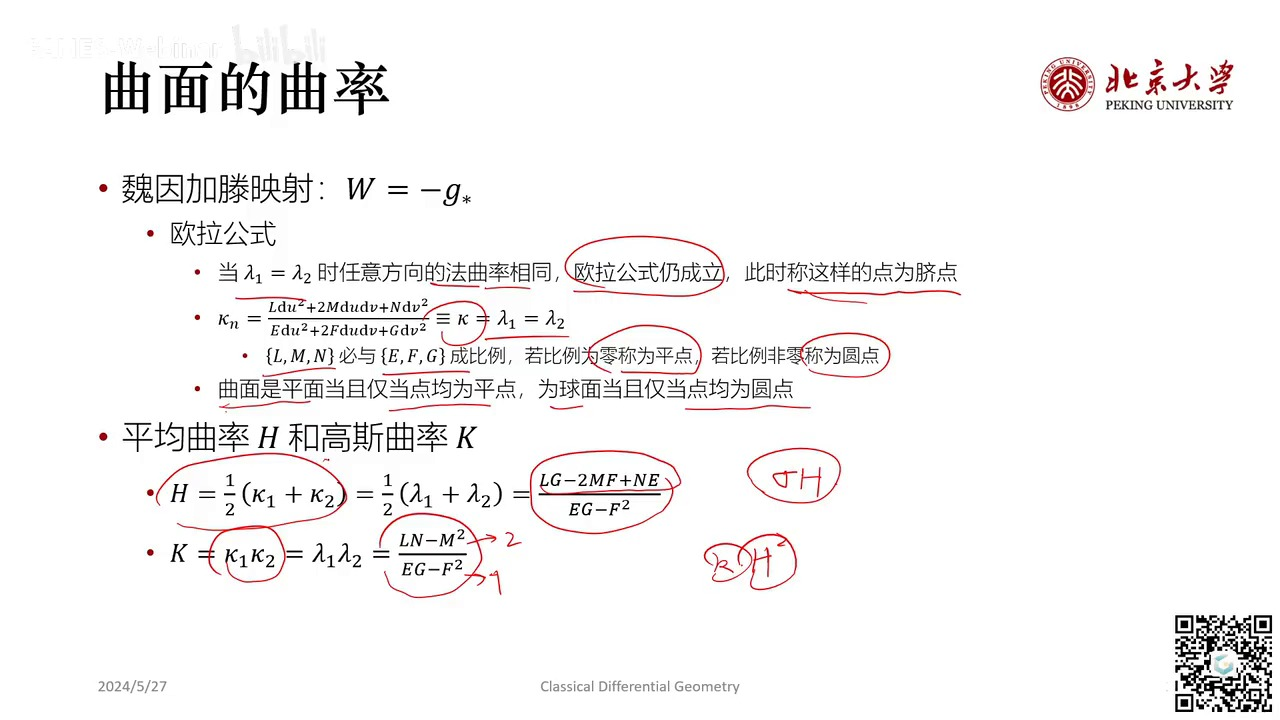
\includegraphics[width=0.92\textwidth]{figures/fig_26_mean_gauss.jpg}
\caption{脐点，以及平均曲率与高斯曲率\vtag}
\end{figure}
\srcnote{01:09:00--01:09:15}
\end{minipage}


当 $\lambda_1=\lambda_2$ 时，任意方向的法曲率相同，欧拉公式仍成立，此时称这样的点为脐点：
\begin{equation}
\kappa_n=\frac{L\,\mathrm{d}u^2+2M\,\mathrm{d}u\,\mathrm{d}v+N\,\mathrm{d}v^2}{E\,\mathrm{d}u^2+2F\,\mathrm{d}u\,\mathrm{d}v+G\,\mathrm{d}v^2}\equiv\kappa=\lambda_1=\lambda_2 .
\end{equation}
此时 $(L,M,N)$ 必与 $(E,F,G)$ 成比例：若比例为零称为平点，若比例非零称为圆点。曲面是平面当且仅当点均为平点，为球面当且仅当点均为圆点，这与前面平面和球面的第二基本形定理一致。

平均曲率 $H$ 和高斯曲率 $K$ 都可以写成第一、第二基本形的函数：
\begin{equation}
H=\frac{1}{2}(\kappa_1+\kappa_2)=\frac{1}{2}(\lambda_1+\lambda_2)=\frac{LG-2MF+NE}{2(EG-F^2)},\qquad K=\kappa_1\kappa_2=\lambda_1\lambda_2=\frac{LN-M^2}{EG-F^2}.
\end{equation}

\begin{warningbox}{平均曲率公式中的因子二}
课件上把平均曲率写成 $H=\frac{LG-2MF+NE}{EG-F^2}$，漏掉了分母上的因子 $2$。由 $H=\frac{1}{2}(\lambda_1+\lambda_2)=\frac{1}{2}\operatorname{tr}(\mathrm{I}^{-1}\mathrm{II})$ 可知正确的式子应如上式，分母为 $2(EG-F^2)$。以单位球面为例可以快速检验：两个主曲率的绝对值都是 $1$，平均曲率的绝对值应为 $1$ 而不是 $2$。
\end{warningbox}

\section{曲面论基本定理}

\noindent\begin{minipage}{\textwidth}
\begin{figure}[H]
\centering
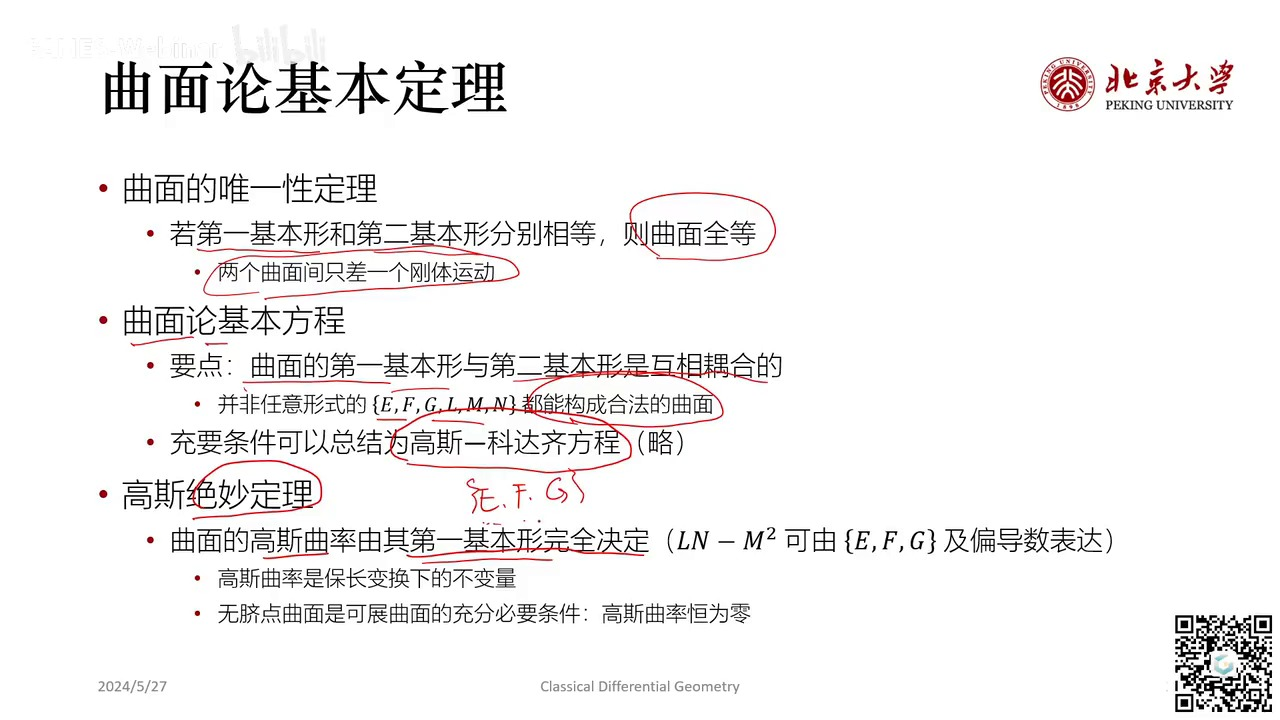
\includegraphics[width=0.92\textwidth]{figures/fig_27_surface_theorem.jpg}
\caption{曲面的唯一性定理、基本方程与高斯绝妙定理\vtag}
\end{figure}
\srcnote{01:10:30--01:10:45}
\end{minipage}


\textbf{曲面的唯一性定理。}若两个曲面的第一基本形和第二基本形分别相等，则曲面全等，两个曲面之间只差一个刚体运动。这与曲线论基本定理是平行的。

\textbf{曲面论基本方程。}要点是：曲面的第一基本形与第二基本形是互相耦合的，并非任意形式的 $\{E,F,G,L,M,N\}$ 都能构成合法的曲面。充要条件可以总结为高斯—科达齐方程，课件从略。

\textbf{高斯绝妙定理。}曲面的高斯曲率由其第一基本形完全决定：$LN-M^2$ 可由 $\{E,F,G\}$ 及其对 $u,v$ 的偏导数表达。讲者强调，这个结论令人惊讶：平均曲率 $H$ 和高斯曲率 $K$ 都是关于弯曲的量，但 $K$ 居然完全由长度来决定。所以高斯曲率是保长变换下的不变量。这意味着可以只在曲面之内考察曲面的弯曲性质，这正是前面所说的现代微分几何，或者说黎曼几何的源头。

\noindent\begin{minipage}{\textwidth}
\begin{figure}[H]
\centering
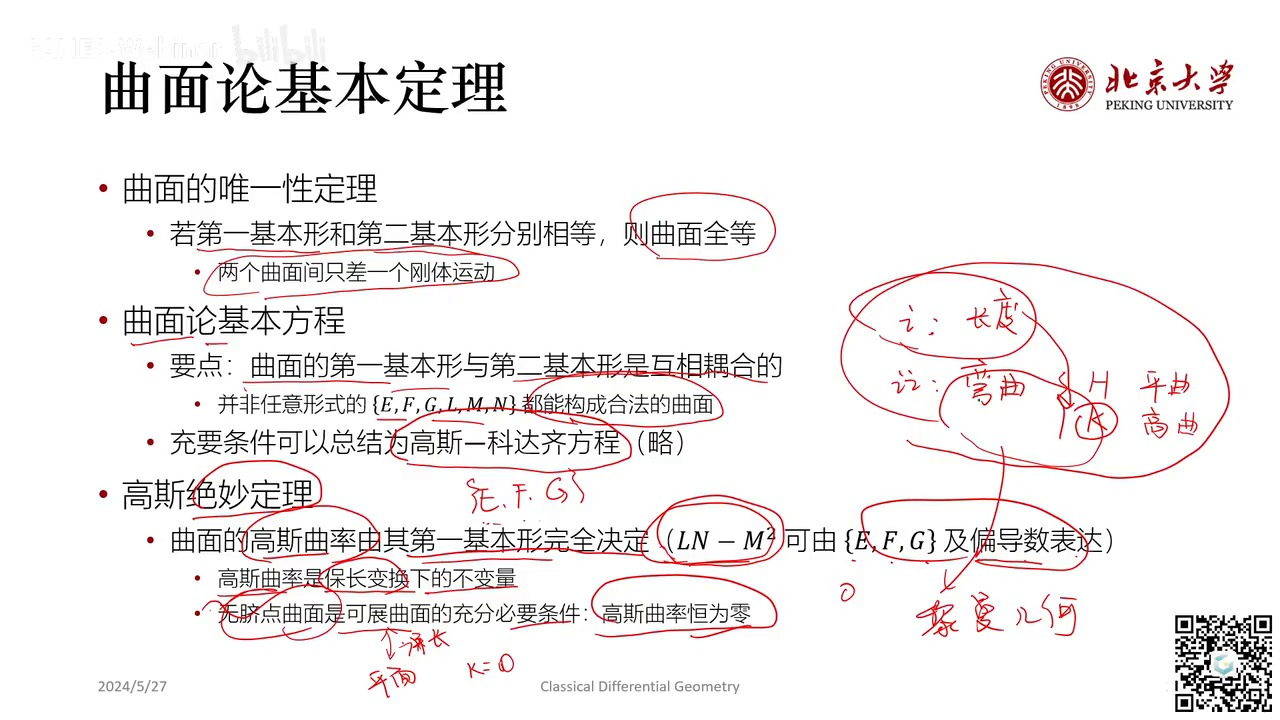
\includegraphics[width=0.92\textwidth]{figures/fig_28_surface_theorem_note.jpg}
\caption{讲者在高斯绝妙定理旁的板书\vtag}
\end{figure}
\srcnote{01:13:45--01:14:00}
\end{minipage}


由此还可以得到：无脐点曲面是可展曲面的充分必要条件是高斯曲率恒为零。高斯曲率为零说明两个主曲率中至少有一个是零。

\begin{practicebox}{用高斯绝妙定理解释生活现象}
讲义作者补充两个例子，读者可以自己想一想：
\begin{enumerate}
\item 为什么地图总有变形？球面的高斯曲率处处为 $1/R^2$，平面为 $0$。若存在保长映射，高斯曲率必须相等，所以不可能把球面无变形地展平。
\item 为什么拿披萨时把边折起来，尖端就不会垂下？披萨饼近似可展，高斯曲率为零；沿一个方向折弯后，该方向主曲率非零，另一个方向主曲率只能为零，于是尖端方向被“拉直”了。
\end{enumerate}
\end{practicebox}

\section{几何连续性}

\subsection{曲线的参数连续性与几何连续性}

\noindent\begin{minipage}{\textwidth}
\begin{figure}[H]
\centering
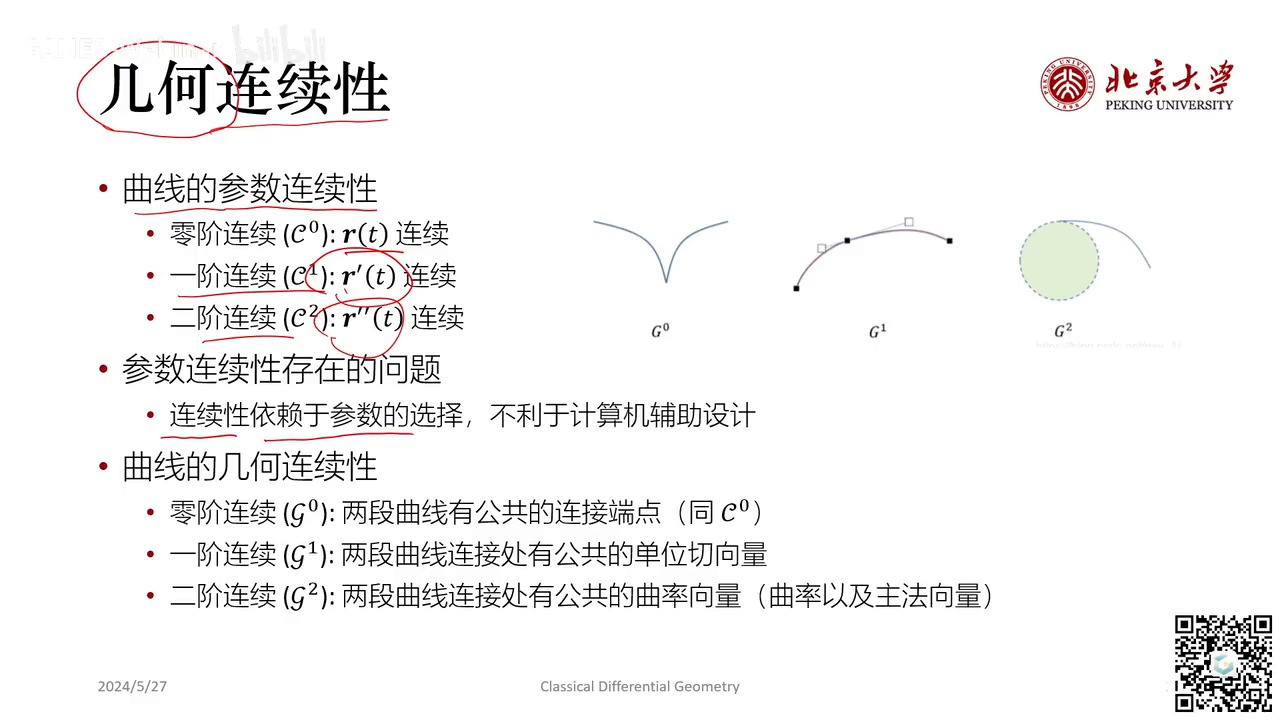
\includegraphics[width=0.92\textwidth]{figures/fig_29_continuity_curve.jpg}
\caption{曲线的参数连续性与几何连续性\vtag}
\end{figure}
\srcnote{01:15:00--01:15:15}
\end{minipage}


最后讲几何连续性。曲线的参数连续性：零阶连续 $C^0$ 指 $\boldsymbol r(t)$ 连续；一阶连续 $C^1$ 指 $\boldsymbol r'(t)$ 连续；二阶连续 $C^2$ 指 $\boldsymbol r''(t)$ 连续。

参数连续性存在的问题是：连续性依赖于参数的选择，不利于计算机辅助设计。讲者举了最简单的例子：球面在极点处参数方程是不连续的，但极点处的球面显然是光滑的，问题只出在参数化上。

因此定义曲线的几何连续性：
\begin{itemize}
\item 零阶连续 $G^0$：两段曲线有公共的连接端点，同 $C^0$；
\item 一阶连续 $G^1$：两段曲线连接处有公共的单位切向量；
\item 二阶连续 $G^2$：两段曲线连接处有公共的曲率向量，即曲率以及主法向量都相同。
\end{itemize}

\noindent\begin{minipage}{\textwidth}
\begin{figure}[H]
\centering
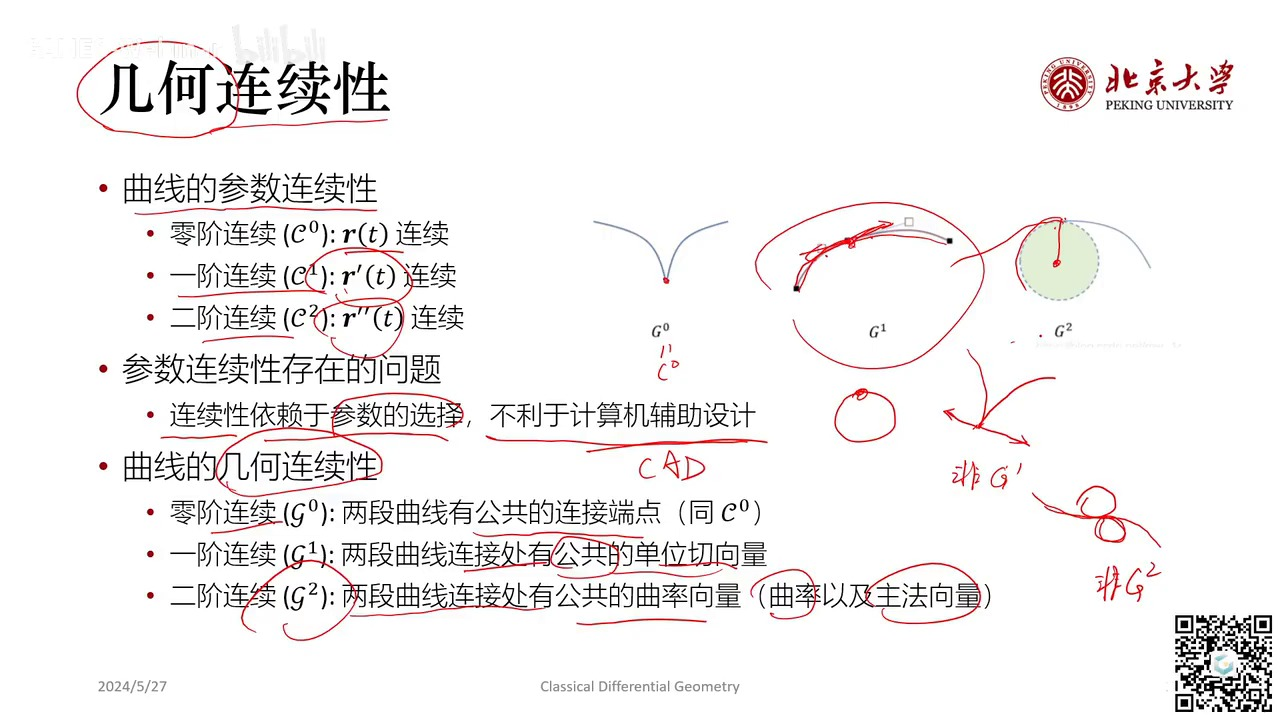
\includegraphics[width=0.92\textwidth]{figures/fig_30_continuity_note.jpg}
\caption{讲者用图示比较 $G^0$、$G^1$ 与 $G^2$ 的连接\vtag}
\end{figure}
\srcnote{01:17:45--01:18:00}
\end{minipage}


\subsection{曲面的连续性}

\noindent\begin{minipage}{\textwidth}
\begin{figure}[H]
\centering
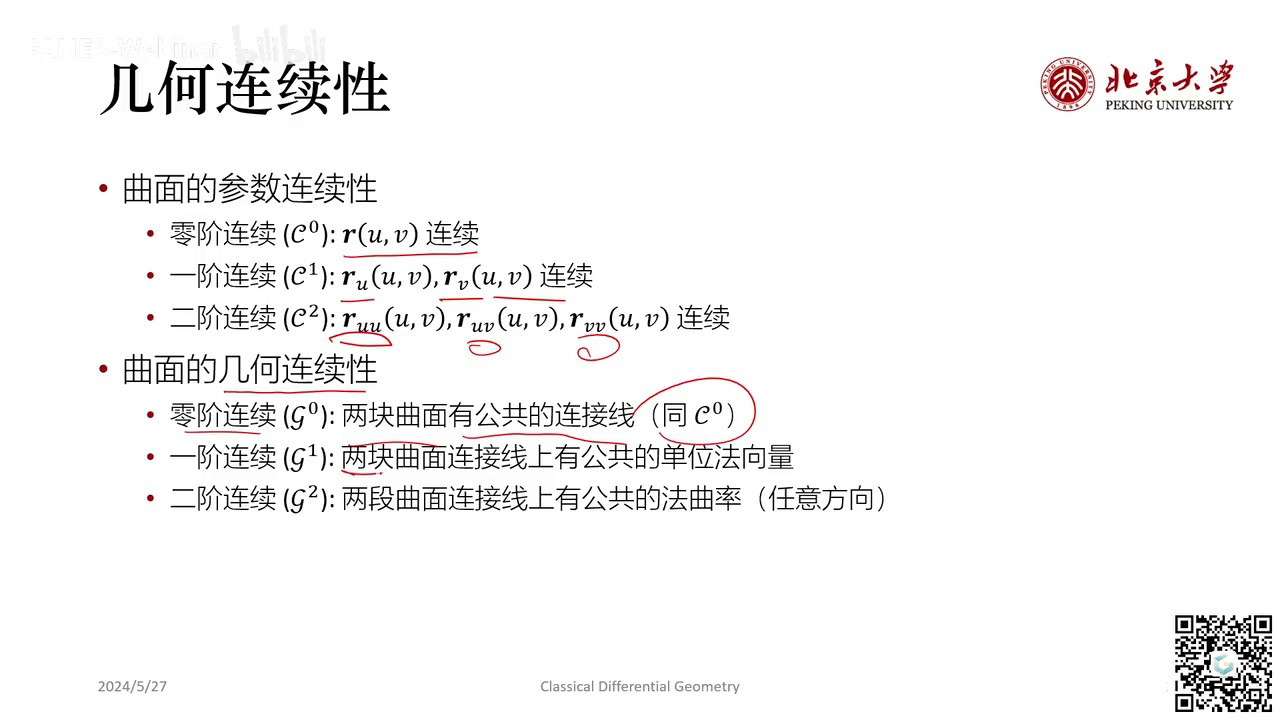
\includegraphics[width=0.92\textwidth]{figures/fig_31_continuity_surface.jpg}
\caption{曲面的参数连续性与几何连续性\vtag}
\end{figure}
\srcnote{01:18:30--01:18:45}
\end{minipage}


对于曲面也是一样。参数连续性：$C^0$ 指 $\boldsymbol r(u,v)$ 连续；$C^1$ 指 $\boldsymbol r_u,\boldsymbol r_v$ 连续；$C^2$ 指 $\boldsymbol r_{uu},\boldsymbol r_{uv},\boldsymbol r_{vv}$ 连续。几何连续性：$G^0$ 指两块曲面有公共的连接线，同 $C^0$；$G^1$ 指两块曲面连接线上有公共的单位法向量；$G^2$ 指两块曲面连接线上有公共的法曲率，并且是任意方向的法曲率都相同。

\begin{warningbox}{$G^1$ 要求法向同向}
有同学问：如果两块曲面在连接处法线一个朝这边、一个朝另一边，算不算几何连续？讲者回答：不算。几何连续更多地对应肉眼直觉，你直觉上觉得它不够连续，它就一定不是几何连续的。若只是参数化方式使单位法向量朝向了相反方向，需要让两块曲面的参数化属性相同（定向一致）再判断。
\end{warningbox}

讲者最后指出，曲面的几何二阶连续是要求非常非常高的性质，因为它要求连接线上每一点、每一个切方向的法曲率都一致。

\section{小结}

讲者说，今天大体介绍了曲线和曲面的相关定理。回顾全讲：曲线用弧长参数化后，切向量的变化给出曲率，次法向量的变化给出挠率，Frenet 公式把三者联系起来，而曲率和挠率完全决定曲线的形状。曲面用第一基本形度量长度、角度和面积，用第二基本形度量弯曲；法曲率是二者之比，其最大最小值即主曲率，乘积与平均分别是高斯曲率与平均曲率。高斯绝妙定理说明高斯曲率是内蕴的。最后，几何连续性用与参数化无关的方式描述曲线和曲面拼接的光滑程度，这是计算机辅助设计中的基本概念。

\begin{knowledgebox}{下一步}
讲义作者补充：本讲是“古典”的、外蕴的、光滑的微分几何。在图形学中，曲面通常以三角网格表示，需要把这里的概念离散化，例如用余切公式近似平均曲率、用角亏近似高斯曲率，这就是离散微分几何的内容。
\end{knowledgebox}

\end{document}
